%%%%%%%%%%%%%%%%%%%%%%%%%%%%%%%%%%%%%%%%%%%%%%%%%%%%%%%%%%%%%%%%%%%%%%%%%%%%%%%%
% Learning and discovering chaotic dynamics from sparse, noisy observations
% Built on the RGU report template (latex_template/RGU_Thesis_Template_2026).
%%%%%%%%%%%%%%%%%%%%%%%%%%%%%%%%%%%%%%%%%%%%%%%%%%%%%%%%%%%%%%%%%%%%%%%%%%%%%%%%
\documentclass{template}
\usepackage{graphicx,parskip,appendix,float}
\usepackage[ruled,vlined,linesnumbered]{algorithm2e}
\usepackage{url,amsmath,amssymb,amsthm,bm,mathtools,listings,pdfpages,caption,subcaption,multicol,datetime,rotating,booktabs,multirow,siunitx}
\usepackage{csquotes}
\usepackage{xcolor}
\usepackage[style=authoryear,giveninits,backend=biber,maxcitenames=2,uniquelist=false]{biblatex}
\addbibresource{references.bib}
\usepackage[pagebackref=false,pdffitwindow=true]{hyperref}
\usepackage{cleveref}

\hypersetup{
    pdftitle    = {Learning and Discovering Chaotic Dynamics from Sparse, Noisy Observations},
    pdfauthor   = {Paul Christopher Aime},
    pdfsubject  = {Data-driven identification of dynamical systems},
    pdfkeywords = {system identification, SINDy, neural ODE, multiple shooting, chaos, uncertainty quantification},
    colorlinks  = true, anchorcolor = blue, filecolor = blue, urlcolor = blue,
    linkcolor   = blue, citecolor = blue,
}

\graphicspath{{../results/figures/}}
\DeclareGraphicsExtensions{.pdf,.png}
\sloppy

\theoremstyle{plain}
\newtheorem{proposition}{Proposition}[chapter]
\newtheorem{lemma}[proposition]{Lemma}
\theoremstyle{definition}
\newtheorem{definition}[proposition]{Definition}
\theoremstyle{remark}
\newtheorem{remark}[proposition]{Remark}

\newcommand{\R}{\mathbb{R}}
\newcommand{\E}{\mathbb{E}}
\newcommand{\Th}{\Theta}
\newcommand{\Xib}{\bm{\Xi}}
\newcommand{\tc}{t_{\mathrm{char}}}
\newcommand{\dto}{\Delta t_{\mathrm{obs}}}
\newcommand{\lmax}{\lambda_{\max}}
\newcommand{\norm}[1]{\left\lVert #1\right\rVert}
\newcommand{\supp}{\operatorname{supp}}
\newcommand{\vpt}{\mathrm{VPT}}

\begin{document}

\title{\LARGE Learning and Discovering Chaotic Dynamics\\ from Sparse, Noisy Observations}
\author{Paul Christopher Aim\'e}
\rpttype{Independent Research Project\\[4pt]{\normalfont\small\itshape Sparse regression, neural ODEs and the landscape of trajectory matching}}
\degreetitle{Computer Engineering (G\'enie Informatique, GI5)}
\institution{\'Ecole Nationale des Sciences Appliqu\'ees de Marrakech\\ Universit\'e Cadi Ayyad, Morocco}
\submitdate{August 2026}

\beforeabstract

\prefacesection{Abstract}
We study how well data-driven methods recover the governing equations of chaotic systems, and forecast their trajectories, from short records that are sparsely sampled and corrupted by noise. The benchmarks are Lorenz-63 and a four-species competitive Lotka--Volterra model with a strange attractor, with a predator--prey model as a non-chaotic control. Measured in units of a characteristic period, the two chaotic systems have the same Lyapunov time, so a single grid of sampling intervals probes both at comparable resolution.

On identical data and with an identical, held-out model-selection rule, we compare dense least squares, SINDy with finite-difference and Savitzky--Golay derivatives, weak-form SINDy, a black-box neural ODE and a sparse-library neural ODE. The last is fitted by differentiating through a Runge--Kutta integrator. Its training combines a Levenberg--Marquardt flow-map stage, quasi-Newton multiple shooting with joint state estimation and continuation in the window length, multistart, and sequential thresholding with trajectory-matching refits.

Exact two-dimensional slices of the trajectory-matching loss show how single shooting degenerates into a flat surface with a needle-like minimum. Gradient norms grow exponentially with the horizon (rate $0.68$ against $\lambda_{\max}=0.91$). In random restarts, short-window multiple shooting brings every start to the same accurate solution, while single shooting over four time units brings none.

With about four samples per oscillation and $1\%$ noise, the sparse neural ODE recovers the Lorenz equations with a median coefficient error of $0.05$, where all derivative-based and weak-form estimators fail. It also gives the longest in-distribution valid prediction times at every sampling interval at this noise level. Black-box neural ODEs yield dense distilled equations, and their forecasts fail immediately from initial conditions off the attractor. For the Lotka--Volterra model, the library matrix has a condition number of order $10^4$ on the data, and no estimator recovers the coefficients from noisy records.

Among the uncertainty estimates, the bootstrap of the weak regression is the best calibrated (90\% interval coverage $0.87$--$0.93$). Bagging the sparse neural ODE gives the lowest CRPS but over-confident intervals. Deep ensembles flag distribution shift; Monte Carlo dropout does not.

\vspace{1em}\noindent\textbf{Keywords:} system identification, sparse regression, SINDy, weak formulation, neural ODEs, multiple shooting, nonconvex optimisation, chaos, uncertainty quantification.


\vspace{0.8em}\noindent{\small\emph{Preprint v1: neural models are evaluated on a sub-grid; the full GPU grid is planned for v2.}}


\afterabstract
\afterpreface
\pagenumbering{arabic}

\chapter{Introduction}\label{ch:intro}

Many physical, biological and engineered systems are described by an autonomous ordinary differential equation
\begin{equation}\label{eq:ode}
  \dot{x}(t) = f\big(x(t)\big), \qquad x(t)\in\R^d,
\end{equation}
whose right-hand side is unknown or only partly known, while some of its trajectories can be measured. Two tasks follow from such measurements. The first is \emph{equation discovery}: recover a closed-form expression for $f$, ideally with the correct set of active terms. The second is \emph{forecasting}: produce a model whose trajectories track the true ones for as long as the dynamics permit, and whose long-run behaviour reproduces the statistics of the true attractor. For chaotic systems the second task has a hard limit. Errors grow on average like $e^{\lmax t}$, so no model, not even the true one started from an imperfect state, predicts beyond a few Lyapunov times $\lmax^{-1}$.

Sparse regression on a library of candidate functions, popularised as SINDy \parencite{brunton2016sindy}, solves the discovery problem remarkably well when the state is densely sampled and nearly noise-free. Its weak point is the time derivative. Finite differences amplify measurement noise by a factor of order $\dto^{-1}$ and are biased by $O(\dto^2)$ when the sampling is coarse. Two families of remedies have emerged. Weak (integral) formulations move the derivative onto smooth test functions \parencite{schaeffer2017integral,reinbold2020weak,messenger2021wsindy}. Integration-based formulations compare model trajectories with the data directly, which is the approach of neural ordinary differential equations \parencite{chen2018node} and of their hybrid, library-based variants \parencite{rackauckas2020ude,goyal2022rk4sindy}.

Integration-based fitting removes the need for derivatives but replaces a convex least-squares problem by a nonconvex one. For a chaotic flow, the sensitivity of a trajectory to its parameters grows exponentially with the integration horizon. The resulting loss surface is rough, with many local minima and gradients whose magnitude spans many orders \parencite{ribeiro2020smoothness}. Whether a neural or hybrid model can be trusted therefore depends as much on the optimiser as on the model class. The same holds for uncertainty. An ensemble of models is only useful if its spread tells us when the forecast, or the identified equation, should not be believed.

This report is a controlled study of these questions on two chaotic benchmarks: the Lorenz-63 system \parencite{lorenz1963} and a four-species competitive Lotka--Volterra (LV) model with a strange attractor \parencite{vano2006chaos}. A classical two-species predator--prey model serves as a non-chaotic control. The contributions are as follows.
\begin{enumerate}
  \item \textbf{A matched benchmark.} Five estimators are compared on identical data, library and model-selection rule over a grid of sampling intervals and noise levels: dense least squares, SINDy with finite-difference and Savitzky--Golay derivatives, weak SINDy, a black-box neural ODE and a sparse-library neural ODE. Time is expressed in units of a characteristic period, in which both chaotic systems have nearly the same Lyapunov time, so one grid probes them at comparable resolution.
  \item \textbf{An analysis of the optimisation problem.} We compute exact two-dimensional slices of the trajectory-matching loss and measure how gradient norms grow with the horizon. We then quantify basins of attraction by random restarts, which isolates three devices that make integration-based identification reliable: multiple shooting, continuation in the window length, and multistart.
  \item \textbf{A sparse-library neural ODE that works at coarse sampling.} It combines a Levenberg--Marquardt flow-map stage, quasi-Newton multiple shooting with joint state estimation, and sequential thresholding with trajectory-matching refits. At a sampling interval of about $4$ observations per oscillation, where every derivative-based and weak-form estimator fails, it recovers the exact Lorenz equations.
  \item \textbf{An assessment of uncertainty and generalisation.} Bootstrap ensembles of sparse models, deep ensembles and Monte Carlo dropout are scored with proper scoring rules on in-distribution and out-of-distribution initial conditions. We also report the conditioning of the library on the data, which explains when equation recovery is impossible regardless of the estimator.
\end{enumerate}

\Cref{ch:related} reviews related work. \Cref{ch:framework} develops the mathematical framework: the error structure of derivative-based and weak estimators, the sensitivity analysis of trajectory matching, and the uncertainty models. \Cref{ch:method} details the protocol and algorithms, \cref{ch:experiments} reports the experiments, and \cref{ch:conclusion} concludes. All code is written in Python with NumPy, SciPy and PyTorch, and is organised as executed Jupyter notebooks.

\chapter{Related Work}\label{ch:related}

\paragraph{Sparse regression for equation discovery.}
SINDy \parencite{brunton2016sindy} writes $f(x)=\Th(x)^\top\Xib$ for a library $\Th$ of candidate functions and estimates a sparse $\Xib$ by sequentially thresholded least squares (STLSQ). \textcite{zhang2019convergence} showed that STLSQ converges to a local minimiser of an $\ell_0$-penalised least-squares objective in finitely many steps. The method has been extended to partial differential equations \parencite{rudy2017pdefind} and to unknown coordinates \parencite{champion2019coordinates}. Model selection has been addressed with information criteria \parencite{mangan2017model}. A widely used implementation is PySINDy \parencite{kaptanoglu2022pysindy}. Noise robustness is the main weakness of the derivative-based formulation. Integral formulations \parencite{schaeffer2017integral} and weak formulations with compactly supported test functions \parencite{reinbold2020weak,messenger2021wsindy} remove the pointwise derivative and are, to our knowledge, the most noise-robust classical variants.

\paragraph{Uncertainty in sparse identification.}
Ensemble-SINDy \parencite{fasel2022esindy} bootstraps the regression and reports inclusion probabilities for every library term. Bayesian alternatives place sparsifying priors on $\Xib$ \parencite{hirsh2022priors}. Both quantify uncertainty in the coefficients. Neither, on its own, says how that uncertainty propagates through a chaotic flow.

\paragraph{Integration-based identification and neural ODEs.}
Neural ODEs \parencite{chen2018node,kidger2021thesis} parameterise $f$ by a neural network and fit it by differentiating through a numerical integrator. Universal differential equations \parencite{rackauckas2020ude} mix known physics with learned terms. RK4-SINDy \parencite{goyal2022rk4sindy} embeds a sparse library inside a Runge--Kutta step to avoid derivative estimation. \textcite{rudy2019denoising} estimate the noise and the dynamics jointly under time-stepping constraints, which is close in spirit to the latent shooting states used here.

\paragraph{Multiple shooting and the smoothness of the loss.}
Multiple shooting \parencite{bock1984multiple} splits a trajectory into windows with free initial states coupled by continuity conditions. It has long been used for parameter estimation in nonlinear and chaotic systems \parencite{voss2004identification,peifer2007multiple}. \textcite{ribeiro2020smoothness} analysed why simulation-error objectives become non-smooth for chaotic systems as the horizon grows. \textcite{turan2022multiple} showed that multiple shooting improves the training of neural differential equations on oscillatory data. Curriculum strategies that lengthen the horizon during training are related to curriculum learning \parencite{bengio2009curriculum}.

\paragraph{Forecasting chaotic systems and benchmarks.}
Data-driven forecasting of chaotic dynamics is commonly evaluated by the valid prediction time, measured in Lyapunov times \parencite{pathak2018reservoir,vlachas2020backprop}. \textcite{gilpin2021chaos} assembled a large benchmark of chaotic systems. Loss surfaces of neural networks are often visualised with filter-normalised random directions \parencite{li2018landscape}. Deep ensembles \parencite{lakshminarayanan2017ensembles} and Monte Carlo dropout \parencite{gal2016dropout} are standard baselines for predictive uncertainty, scored here with proper scoring rules \parencite{gneiting2007scoring}.

\paragraph{Position of this work.}
Most comparisons of discovery methods vary noise at a fixed, dense sampling rate, and evaluate either equations or forecasts but not both. Here the sampling interval is the primary axis. We measure equations, short-term forecasts, long-term statistics and calibrated uncertainty on the same models, and we connect the success or failure of integration-based fitting to the measured geometry of its loss surface.

\chapter{Mathematical Framework}\label{ch:framework}

\section{Problem statement}

Let $x:[0,T_e]\to\R^d$ solve \eqref{eq:ode} for $E$ experiments $e=1,\dots,E$ with initial states $x^{(e)}(0)$. We observe
\begin{equation}\label{eq:obs}
  y^{(e)}_k = x^{(e)}(t^{(e)}_k) + \eta^{(e)}_k,\qquad \eta^{(e)}_k \overset{\text{iid}}{\sim}\mathcal N\big(0,\varepsilon^2\Sigma_x\big),\qquad t^{(e)}_{k+1}-t^{(e)}_k=\dto,
\end{equation}
where $\Sigma_x=\operatorname{diag}(\sigma_1^2,\dots,\sigma_d^2)$ collects the variances of the coordinates on the attractor and $\varepsilon$ is the relative noise level.

\paragraph{Library representation.} Let $\theta:\R^d\to\R^p$ be the vector of all monomials of total degree at most two, $p=\binom{d+2}{2}$, ordered as $1, x_1,\dots,x_d, x_1^2, x_1x_2,\dots,x_d^2$. All systems in this study satisfy
\begin{equation}\label{eq:library}
  f(x) = \Xib^\top\theta(x),\qquad \Xib\in\R^{p\times d},
\end{equation}
with a sparse coefficient matrix whose support $\supp(\Xib)=\{(k,j):\xi_{kj}\neq 0\}$ is known for scoring. Equation discovery is the estimation of $\Xib$. We score it by the relative error $\norm{\hat\Xib-\Xib}_F/\norm{\Xib}_F$ and by the precision, recall and $F_1$ score of $\supp(\hat\Xib)$.

\paragraph{Nondimensionalisation.} Coefficients of different monomials carry different physical units, so a single sparsity threshold is meaningless in raw coordinates. We work with $z=S^{-1}x$, $S=\operatorname{diag}(s_1,\dots,s_d)$, where $s_i$ is the root mean square of the noisy data, and with $\tau=t/\tc$.

\begin{lemma}[Support invariance]\label{lem:scaling}
For a monomial with exponent vector $\pi_k\in\mathbb N^d$ put $c_k=\prod_i s_i^{\pi_{ki}}$ and $C=\operatorname{diag}(c_1,\dots,c_p)$. Then $z$ satisfies $dz/d\tau=\tilde\Xib^\top\theta(z)$ with
\begin{equation}
  \tilde\Xib = \tc\, C\,\Xib\,S^{-1},
\end{equation}
so $\supp(\tilde\Xib)=\supp(\Xib)$.
\end{lemma}
\begin{proof}
$\theta_k(Sz)=c_k\theta_k(z)$ for every monomial, hence $\dot z = S^{-1}\Xib^\top C\theta(z)$, and the chain rule gives the factor $\tc$. Both $C$ and $S$ are diagonal with positive entries.
\end{proof}
Centring the data, $z=S^{-1}(x-\mu)$, would instead mix monomials of different degree and destroy the support, so we never centre.

\paragraph{Identifiability.} On a finite record, the coefficients are determined only through the matrix $\Th(Z)\in\R^{N\times p}$ whose rows are $\theta(z_k)^\top$. If $\sigma_{\min}$ denotes its smallest singular value divided by $\sqrt N$, any estimator that is linear in an estimate $\hat{\dot Z}$ of the derivatives satisfies, to first order,
\begin{equation}\label{eq:ident}
  \norm{\delta\tilde\Xib}_F \lesssim \frac{1}{\sigma_{\min}}\Big(\frac{1}{N}\norm{\delta\dot Z}_F^2\Big)^{1/2}.
\end{equation}
A trajectory confined to a thin attractor makes some monomials nearly collinear, so $\sigma_{\min}$ can be tiny. This is a property of the data, not of the estimator, and \cref{sec:exp-data} shows that it governs the four-species LV model.

\section{Estimators built on derivative surrogates}

STLSQ \parencite{brunton2016sindy} approximately solves
\begin{equation}\label{eq:l0}
  \min_{\tilde\Xib}\ \norm{\hat{\dot Z}-\Th(Z)\tilde\Xib}_F^2 + \lambda^2\norm{\tilde\Xib}_0
\end{equation}
by alternating a least-squares solve on the current support with the removal of all coefficients with $|\tilde\xi_{kj}|<\lambda$. It terminates in finitely many sweeps, because the support can only shrink \parencite{zhang2019convergence}.

\paragraph{Finite differences.} For the central difference $D_k=(y_{k+1}-y_{k-1})/(2\dto)$,
\begin{equation}\label{eq:fd}
  D_k = \dot x(t_k) + \frac{\dto^2}{6}\,x^{(3)}(t_k) + O(\dto^4) + \frac{\eta_{k+1}-\eta_{k-1}}{2\dto}.
\end{equation}
The noise term has covariance $\varepsilon^2\Sigma_x/(2\dto^2)$, which explodes at dense sampling. The truncation term is controlled by the dominant angular frequency $\omega=2\pi/\tc$: for a component oscillating like $e^{i\omega t}$, the relative bias is $(\omega\dto)^2/6$. On our grid $\dto/\tc\in\{\tfrac{1}{75},\tfrac{1}{15},\tfrac{2}{15},\tfrac{4}{15}\}$, so this bias is $0.12\%$, $2.9\%$, $11.7\%$ and $47\%$ of the derivative. A $47\%$ systematic error in the regression targets cannot be removed by any sparsity pattern, which explains why all derivative-based estimators fail at the coarsest sampling.

\paragraph{Savitzky--Golay derivatives.} A local polynomial fit of degree three over $w$ samples \parencite{savitzky1964} reduces the noise gain by a factor of about $w^{3/2}$. In exchange it adds a bias that grows with the window length $w\dto$ relative to $\tc$. The window is a hyper-parameter, and we select it on held-out data.

\section{Weak formulation}

Let $\phi\in C^{q}(\R)$ be supported on $[t_c-H,t_c+H]$. Multiplying \eqref{eq:ode} by $\phi$ and integrating by parts removes the derivative from the data:
\begin{equation}\label{eq:weak}
  -\int \dot\phi(t)\,x(t)\,dt = \Big(\int\phi(t)\,\theta\big(x(t)\big)\,dt\Big)^{\!\top}\Xib .
\end{equation}
With $K$ test functions $\phi_k$ and the trapezoidal rule on the samples, this yields a linear system $G\Xib=B$ with $G_{kj}\approx\int\phi_k\theta_j(y)$ and $B_{ki}\approx-\int\dot\phi_k y_i$, which we solve by STLSQ \parencite{messenger2021wsindy}. We use $\phi(t)=\big(1-((t-t_c)/H)^2\big)^{4}$, whose first three derivatives vanish at the endpoints of its support.

\begin{proposition}[Quadrature order]\label{prop:quad}
Let $g=\phi\,\theta_j(x)$ be smooth on the support of $\phi$, and let $g^{(m)}$ vanish at both endpoints for $m\le q$. Then the trapezoidal rule with step $\dto$ has error $O\big(\dto^{2\lfloor q/2\rfloor+2}\big)$. For $q=3$ this is $O(\dto^6)$, against $O(\dto^2)$ for the central difference \eqref{eq:fd}.
\end{proposition}
\begin{proof}
By the Euler--Maclaurin formula, the error is $\sum_{j\ge1}\frac{B_{2j}}{(2j)!}\dto^{2j}\big[g^{(2j-1)}\big]_{t_c-H}^{t_c+H}$ plus a remainder of the same order as the first omitted term. Every bracket with $2j-1\le q$ vanishes.
\end{proof}

Measurement noise enters \eqref{eq:weak} through averages $\int\dot\phi\,\eta$. Their variance is $O(\varepsilon^2\dto/H)$ rather than $O(\varepsilon^2/\dto^2)$, so the weak form is both higher order and noise-averaging. Its limitation is that \cref{prop:quad} is asymptotic: when $\dto$ is a sizeable fraction of $\tc$, the integrand is not resolved and the quadrature error is $O(1)$.

\section{Trajectory matching and the geometry of its loss}\label{sec:tm}

Integration-based methods avoid derivative surrogates altogether. Let $\Phi^t_\vartheta(x_0)$ denote the flow of a parametric field $f_\vartheta$. This is either the library model $f_{\Xib}(x)=\Xib^\top\theta(x)$ or a neural network $f_\vartheta=g_\vartheta$. Single shooting minimises
\begin{equation}\label{eq:ss}
  \mathcal L_T(\vartheta) = \frac{1}{n}\sum_{k=1}^{n}\norm{\Phi^{t_k}_\vartheta(x_0)-y_k}^2_{\Sigma_x^{-1}},\qquad t_n=T .
\end{equation}

\paragraph{Sensitivities grow exponentially.} The parameter sensitivity $U(t)=\partial\Phi^t_\vartheta(x_0)/\partial\vartheta$ obeys the variational equation
\begin{equation}\label{eq:sens}
  \dot U = J_\vartheta\big(x(t)\big)\,U + \partial_\vartheta f_\vartheta\big(x(t)\big),\qquad U(0)=0,
\end{equation}
with $J_\vartheta=\partial_x f_\vartheta$. By variation of constants, $U(t)=\int_0^t M(t,s)\,\partial_\vartheta f\,ds$, where $M$ is the state-transition matrix of the linearised flow. On a chaotic attractor, the multiplicative ergodic theorem gives $\norm{M(t,s)}\approx e^{\lmax(t-s)}$ for typical orbits, hence $\norm{U(t)}\sim e^{\lmax t}/\lmax$.

\begin{proposition}[Curvature and basin width of single shooting]\label{prop:basin}
Near the true parameter $\vartheta^\star$ and in the noise-free case, the Gauss--Newton Hessian of \eqref{eq:ss} is $\mathcal H_T=\frac{2}{n}\sum_k U(t_k)^\top\Sigma_x^{-1}U(t_k)$. Its largest eigenvalue grows like $e^{2\lmax T}$, and so does $\norm{\nabla\mathcal L_T}$ divided by the parameter error. The quadratic model of $\mathcal L_T$ is accurate only while the linearisation $\Phi^t_{\vartheta}\approx\Phi^t_{\vartheta^\star}+U\delta\vartheta$ holds over the whole horizon, that is, for $\norm{\delta\vartheta}\lesssim \delta_{\rm nl}\,e^{-\lmax T}$, where $\delta_{\rm nl}$ is the scale at which the flow stops being linear. The region in which descent methods behave as on a convex problem therefore shrinks exponentially with $T$.
\end{proposition}
The statement is a heuristic consequence of \eqref{eq:sens}, not a theorem with constants. \Cref{sec:exp-landscape} checks it numerically: the median gradient norm grows at a rate close to $\lmax$, and the exact loss surfaces become rough on scales that shrink with $T$.

\paragraph{Multiple shooting.} Let $S=\{S_i\}$ be free \emph{shooting states}, one per observation time. Multiple shooting with windows of $K$ observation intervals minimises
\begin{equation}\label{eq:ms}
  \mathcal J_K(\vartheta,S) = \frac{1}{|\mathcal W|K}\sum_{i\in\mathcal W}\sum_{k=1}^{K}\norm{\Phi^{t_{i+k}-t_i}_\vartheta(S_i)-y_{i+k}}^2_{\Sigma_x^{-1}} + \frac{w}{N}\sum_{i}\norm{S_i-y_i}^2_{\Sigma_x^{-1}},
\end{equation}
where $\mathcal W$ indexes the windows that do not straddle two experiments. A window starting at $S_i$ and ending beyond $t_{i+1}$ must reproduce the data that later states are tied to, so continuity holds in the limit, while the data term penalises states that drift from the observations. This form, with all windows active and one state per sample, makes $S$ a denoised estimate of the trajectory, in the spirit of \textcite{rudy2019denoising}. Because every residual involves at most $K\dto$ of integration, the sensitivities in \eqref{eq:ms} are bounded by $e^{\lmax K\dto}$ independently of the record length. The record length only adds residuals, that is, information. Single shooting is the special case of one window with $S_0$ fixed.

\paragraph{Continuation in the window length.} The case $K=1$ with $S$ fixed at the data is a one-step flow-map regression,
\begin{equation}\label{eq:flowmap}
  \min_{\Xib}\ \sum_i\norm{\Phi^{\dto}_{\Xib}(y_i)-y_{i+1}}^2_{\Sigma_x^{-1}} .
\end{equation}
For small $\dto$, $\Phi^{\dto}_{\Xib}(y)=y+\dto\,\Xib^\top\theta(y)+O(\dto^2)$ is nearly linear in $\Xib$, so \eqref{eq:flowmap} is a mildly nonlinear least-squares problem with a wide basin. Our sparse-library estimator solves \eqref{eq:flowmap} first. It then increases $K$ geometrically ($K=1,2,3,5,8,\dots$), and every stage starts inside the basin found at the previous one. This is a homotopy from a nearly convex problem to the full one, consistent with \cref{prop:basin}.

\section{Uncertainty models}\label{sec:uq-theory}

We compare four constructions of a predictive distribution. Each yields $M$ vector fields $\{f^{(m)}\}$, and forecasts are obtained by integrating each of them from the same initial condition.
\begin{itemize}
  \item \textbf{Bootstrap of the weak regression (E-SINDy).} Rows of $(G,B)$ are resampled with replacement and STLSQ is rerun with the selected threshold \parencite{fasel2022esindy}. Inclusion probabilities $\hat P(\xi_{kj}\neq0)$ summarise uncertainty about the support.
  \item \textbf{Window bagging (N2).} The set $\mathcal W$ in \eqref{eq:ms} is resampled with replacement for each member of the sparse-library model.
  \item \textbf{Deep ensembles (N1).} Independent initialisations and minibatch streams of the black-box model \parencite{lakshminarayanan2017ensembles}.
  \item \textbf{Monte Carlo dropout (N1).} With dropout masks $\zeta\sim\mathrm{Bernoulli}(1-p)$ on hidden units \parencite{gal2016dropout}. We draw the mask \emph{once per trajectory} and hold it fixed along the rollout, so each sample $f_{\vartheta,\zeta}$ is an autonomous vector field. Resampling the mask at every Runge--Kutta stage would turn the model into a random dynamical system, whose dispersion reflects injected noise rather than epistemic uncertainty.
\end{itemize}
The predictive distributions are scored by the empirical coverage of central $90\%$ intervals and by the continuous ranked probability score. For a sample $\{X^{(m)}\}$ and outcome $y$ the latter is
\begin{equation}\label{eq:crps}
  \mathrm{CRPS} = \frac{1}{M}\sum_m|X^{(m)}-y| - \frac{1}{2M^2}\sum_{m,m'}|X^{(m)}-X^{(m')}| ,
\end{equation}
a strictly proper score \parencite{gneiting2007scoring}. Both are computed per coordinate, in units of $\sigma_i$, as functions of lead time. We also report the rank correlation between the ensemble spread and the error of the ensemble mean (spread--skill).

\chapter{Methodology}\label{ch:method}

\section{Systems and ground truth}\label{sec:systems}

\Cref{tab:systems} lists the three systems. The four-species model of \textcite{vano2006chaos},
\begin{equation}\label{eq:lv4}
  \dot x_i = r_i x_i\Big(1-\sum_{j=1}^4 a_{ij}x_j\Big),\quad
  r=\begin{pmatrix}1\\0.72\\1.53\\1.27\end{pmatrix},\quad
  A=\begin{pmatrix}1&1.09&1.52&0\\0&1&0.44&1.36\\2.33&0&1&0.47\\1.21&0.51&0.35&1\end{pmatrix},
\end{equation}
leaves the positive orthant invariant and carries a strange attractor with $\lmax\approx0.020$. Every system is quadratic, so its vector field lies exactly in the span of the degree-2 library. Ground truth is computed with the eighth-order Dormand--Prince scheme \parencite{hairer1993solving} (\texttt{scipy.integrate.solve\_ivp}, method \texttt{DOP853}, $\mathrm{rtol}=10^{-10}$, $\mathrm{atol}=10^{-12}$) on a grid of step $\tc/750$.

The characteristic period $\tc$ is the mean interval between successive maxima of the oscillating coordinate. For Lorenz-63 this is $z$, with $\tc=0.75$; for LV4 it is $x_1$, with $\tc\approx 34$, rounded to $35$. Re-estimating $\lmax$ by the method of \textcite{benettin1980lyapunov} with the RK4 step used for learned models gives $0.906$ and $0.019$. Hence $\lmax\tc=0.68$ and $0.67$, so the two chaotic systems have the same predictability horizon in units of their own period. This allows a single sampling grid expressed in $\tc$.

\begin{table}[t]
\centering
\caption{Benchmark systems. $p$ is the library size, $|\supp\Xib|$ the number of active coefficients out of $pd$.}
\label{tab:systems}
\small
\begin{tabular}{lcccccc}
\toprule
system & $d$ & $p$ & $|\supp\Xib|$ & $\tc$ & $\lmax$ & regime \\
\midrule
Lorenz-63, $(\sigma,\rho,\beta)=(10,28,8/3)$ & 3 & 10 & 7/30 & 0.75 & 0.906 & chaotic \\
competitive LV \eqref{eq:lv4} & 4 & 15 & 17/60 & 35 & 0.020 & chaotic \\
predator--prey, $(\alpha,\beta,\delta,\gamma)=(\tfrac23,\tfrac43,1,1)$ & 2 & 6 & 4/12 & 8 & 0 & periodic \\
\bottomrule
\end{tabular}
\end{table}

\section{Experimental design}\label{sec:design}

\paragraph{Training records.} A record has a total length of $\tfrac{80}{3}\tc$ (20 time units, or 18 Lyapunov times, for Lorenz). It consists of $E=4$ independent experiments of $\tfrac{20}{3}\tc$ each. Each experiment starts from a random point of a long reference orbit, displaced by Gaussian noise of $0.5\,\sigma_i$ per coordinate and clipped to the positive orthant for LV. Several short experiments excite directions of the library that a single orbit on the attractor never visits (\cref{sec:exp-data}). The last $20\%$ of every experiment is held out for model selection, and no estimator sees the true coefficients.

\paragraph{Corruption grid.} The records are sub-sampled at $\dto/\tc\in\{\tfrac1{75},\tfrac1{15},\tfrac2{15},\tfrac4{15}\}$, which is $\dto\in\{0.01,0.05,0.1,0.2\}$ for Lorenz, or 75, 15, 7.5 and 3.75 samples per period. Gaussian noise with $\varepsilon\in\{0,1,2,5,10,20\}\%$ is added. Every cell is repeated with 3 seeds, which change both the initial states of the experiments and the noise. The classical estimators run on the full grid, on an irregular-sampling condition and on the predator--prey control. The neural estimators run on a cross-shaped sub-grid: a sampling sweep at $\varepsilon=1\%$ and a noise sweep at $\dto=\tc/15$.

\paragraph{Test sets.}
\begin{itemize}
  \item \emph{In-distribution (ID)}: 16 initial conditions on the attractor, taken from a reference orbit at least $5\tc$ apart.
  \item \emph{Out-of-distribution (OOD)}: 16 initial conditions drawn uniformly in a box extended by $50\%$ of the attractor's span on each side, kept only if their distance to the attractor exceeds 2 in units of $\sigma_i$ (minimum distance 2.0 for Lorenz and 2.5 for LV4).
\end{itemize}
True forecasts cover 15 Lyapunov times. Long-run statistics are compared with a reference orbit of $200\tc$. Every learned model is integrated with the classical RK4 scheme and step $h=\tc/75$, so that differences between models reflect the vector field and not the integrator.

\section{Classical estimators}

\begin{itemize}
  \item \textbf{C1} is dense least squares on central differences (\cref{eq:fd}).
  \item \textbf{C2-FD} and \textbf{C2-SG} are STLSQ on central-difference and Savitzky--Golay derivatives (cubic, window $w\in\{5,7,9,13,17,25\}$).
  \item \textbf{C3} is weak SINDy with test functions $(1-s^2)^4$ of half-width $H\in\{0.1,0.2,0.35,0.5,0.75\}\tc$, admissible only when $H\ge2\dto$, with centres spaced by half the number of samples in $H$.
\end{itemize}
STLSQ uses a ridge term of $10^{-10}$ for numerical stability. The threshold is searched on 24 values log-spaced in $[10^{-4},0.5]\times\max|\tilde\Xib_{\rm OLS}|$.

\paragraph{Model selection.} Every candidate model is scored on the held-out blocks by short rollouts of length $\tc$, started from 24 noisy observations and compared with the noisy data that follow. The selected model is the sparsest one whose error is within $5\%$ (plus an absolute $10^{-4}$) of the best. The same rule selects the thresholds of the neural models. Because the comparison is made against noisy data, the noise floor is common to all candidates and does not bias the ranking.

\section{Neural estimators}

\paragraph{N1: black-box neural ODE.} The field is $f_\vartheta(x)=S\,g_\vartheta\big(S^{-1}(x-\mu)\big)/\tc$, with $g_\vartheta$ a $\tanh$ network with two hidden layers of 64 units. Its output layer is initialised small, so that early rollouts stay bounded. We minimise \eqref{eq:ms} with Adam \parencite{kingma2015adam} over minibatches of 128 windows and the shooting states, using gradient-norm clipping at 1 and a curriculum of window lengths $H\in\{0.1,0.25,0.5,1\}\tc$ (200, 250, 300 and 450 iterations). Learning rates start at $3\cdot10^{-3}$ for the network and $10^{-2}$ for the states, decay by $0.6$ per stage, and follow a cosine schedule in the last stage. Equations are extracted by \emph{symbolic distillation}: STLSQ of $f_\vartheta(S_i)$ on $\theta(S_i)$ over the denoised states, with the usual selection rule.

\paragraph{N2: sparse-library neural ODE.} The field is $f_{\Xib}(x)=S\,\tilde\Xib^\top\theta(S^{-1}x)/\tc$ (\cref{lem:scaling}), fitted by differentiating through the RK4 integrator. \Cref{alg:n2} summarises the procedure. The Levenberg--Marquardt stage \parencite{marquardt1963} uses the exact Jacobian of the one-step residuals with respect to the $pd$ coefficients, obtained by forward-mode automatic differentiation. With Marquardt's diagonal scaling, its steps are invariant to the column scaling of $\Th$, which matters when the library is badly conditioned. The joint stages use full-batch L-BFGS \parencite{liu1989lbfgs} with a strong Wolfe line search over $(\tilde\Xib,S)$. A stage whose final objective is non-finite or higher than its initial value is discarded, and the curriculum stops there. The warm-started variant N2-WS adds the weak-SINDy estimate to the set of initialisations.

\begin{algorithm}[t]
\caption{Sparse-library neural ODE (N2)}\label{alg:n2}
\DontPrintSemicolon
\KwIn{experiments $\{(t^{(e)}_k,y^{(e)}_k)\}$, held-out blocks, initialisations $\mathcal I=\{0,\tilde\Xib_{\rm OLS}\}$ (N2-WS: $\cup\{\tilde\Xib_{\rm WSINDy}\}$)}
\ForEach{$\tilde\Xib_0\in\mathcal I$}{
  $S\leftarrow y$ \tcp*{raw observations; no smoothing}
  $\tilde\Xib\leftarrow$ Levenberg--Marquardt on the flow-map problem \eqref{eq:flowmap}, $S$ fixed\;
  \For{$K = 1,2,3,5,8,\dots,K_{\max}$ \tcp*{$K_{\max}\dto\approx\tc$}}{
    $(\tilde\Xib,S)\leftarrow$ L-BFGS on $\mathcal J_K$ \eqref{eq:ms}, 60 iterations\;
    \lIf{$\mathcal J_K$ non-finite or increased}{restore previous $(\tilde\Xib,S)$ and \textbf{break}}
  }
  score the run by the held-out rollout error\;
}
keep the best run; $\mathcal P\leftarrow\{\tilde\Xib\}$\;
\For{$\lambda$ on 12 values log-spaced in $[10^{-3},10^{-0.4}]\max|\tilde\Xib|$}{
  \Repeat{the support is unchanged (at most 4 sweeps)}{
    zero all $|\tilde\xi_{kj}|<\lambda$; refit the survivors by L-BFGS on $\mathcal J_{K}$ with $S$ fixed\;
  }
  $\mathcal P\leftarrow\mathcal P\cup\{\tilde\Xib\}$ \tcp*{continuation: next $\lambda$ starts here}
}
\KwOut{the sparsest model in $\mathcal P$ within tolerance of the best held-out error}
\end{algorithm}

\section{Metrics}\label{sec:metrics}

\paragraph{Equations.} Relative coefficient error and support $F_1$, as defined in \cref{ch:framework}. A support counts as \emph{exact} when it matches $\supp\Xib$ entry by entry.

\paragraph{Short-term forecasts.} With the normalised error $e(t)=\big(\frac1d\sum_i(\hat x_i-x_i)^2/\sigma_i^2\big)^{1/2}$, the valid prediction time is $\vpt=\lmax\inf\{t:e(t)>0.4\}$, measured in Lyapunov times. We report its mean over the 16 ID and the 16 OOD initial conditions. For a model with the exact vector field, the RK4 discretisation alone limits the VPT to about 11 Lyapunov times on Lorenz.

\paragraph{Long-term statistics.} From a free run of $200\tc$ after a burn-in of $20\tc$ we compute three quantities:
\begin{itemize}
  \item the mean, over coordinates, of the Wasserstein-1 distance $W_1$ between marginal invariant densities, in units of $\sigma_i$;
  \item the relative error of the Benettin estimate of $\lmax$ (renormalisation every 10 steps, $d_0=10^{-8}$, $100\tc$);
  \item the divergence rate, a run being divergent if its state becomes non-finite or exceeds $10^4$ in norm.
\end{itemize}

\section{Implementation}

All code is in Python 3.13. It uses NumPy 2.5 and SciPy 1.18 for simulation and sparse regression, and PyTorch 2.14 in double precision for the neural models. It is organised as six executed notebooks plus a small \texttt{src/} package. The experiments ran on two CPU cores. A sparse-library fit takes 0.5 to 3 minutes, a black-box fit about 2 minutes, and a classical fit with model selection a few seconds. A GPU notebook reruns the full neural grid.

\chapter{Experiments}\label{ch:experiments}

Unless stated otherwise, numbers are medians over the three seeds, coefficient errors are relative Frobenius errors, and valid prediction times (VPT) are in Lyapunov times. Every number in this chapter is exported to \texttt{results/metrics/}.

\section{Data, conditioning and identifiability}\label{sec:exp-data}

\Cref{fig:attractors} shows the reference orbits and \cref{fig:corruption} the observation records at three corruption levels. At $\dto=4\tc/15$ an experiment contains only 25 samples, about four per oscillation. The peaks of the signal are no longer resolved, and an observer would struggle to draw the trajectory between consecutive points.

\begin{figure}[t]
  \centering
  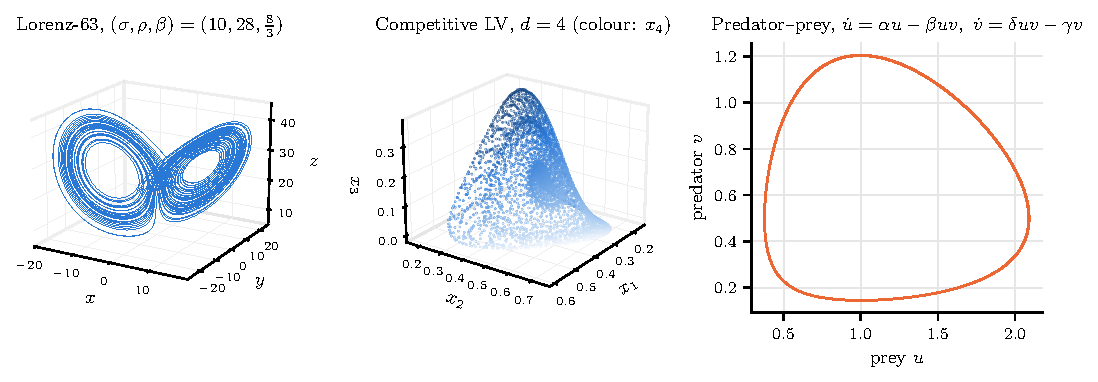
\includegraphics[width=\textwidth]{fig01_attractors}
  \caption{Reference attractors. Left: Lorenz-63. Centre: the four-species competitive Lotka--Volterra model, projected on $(x_1,x_2,x_3)$ and coloured by $x_4$. Right: the periodic predator--prey control.}
  \label{fig:attractors}
\end{figure}

\begin{figure}[t]
  \centering
  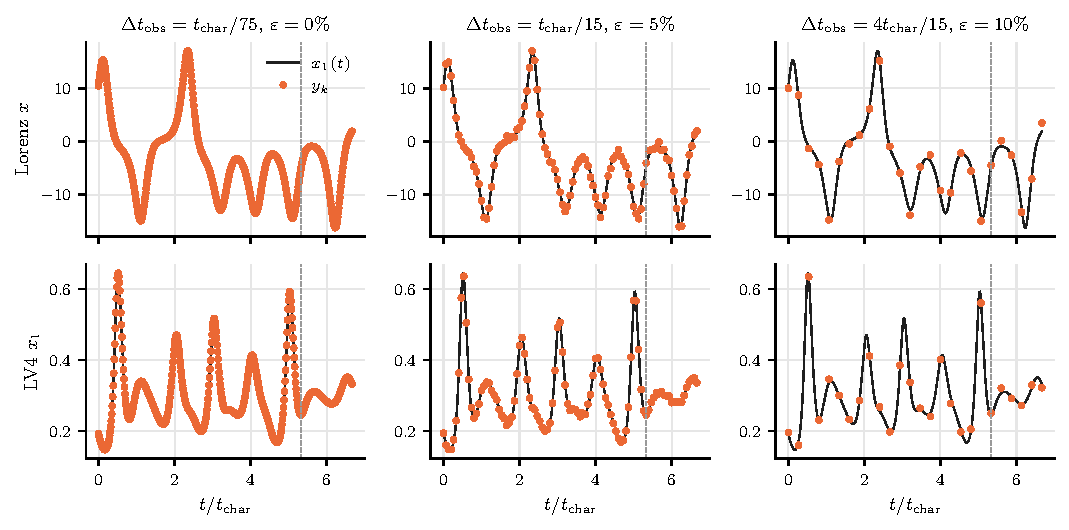
\includegraphics[width=\textwidth]{fig01_corruption}
  \caption{First experiment of a training record at three corruption levels (seed 0). The dashed line separates the fitting block from the held-out block.}
  \label{fig:corruption}
\end{figure}

\Cref{fig:spectrum} reports the singular values of the normalised library matrix $\Th(Z)/\sqrt N$ on noise-free data. For Lorenz-63, $\sigma_{\min}\approx0.025$ and the condition number is about $120$, whether the record is one orbit or four perturbed experiments. The competitive LV model is very different. On a single orbit $\sigma_{\min}=1.6\times10^{-5}$ ($\kappa=2.3\times10^{5}$); four experiments raise it to $1.3\times10^{-4}$ ($\kappa=3.4\times10^{4}$), an eight-fold improvement that is still two orders of magnitude worse than Lorenz. By \eqref{eq:ident}, a derivative error of $1\%$ of the signal can then produce coefficient errors of order one. This is what we observe: on noise-free data the Savitzky--Golay and weak estimators recover the LV4 coefficients to $10^{-4}$ or better, but at $\varepsilon=1\%$ every classical estimator returns coefficient errors between $1.06$ and $1.63$ with either design (\cref{tab:design}). The four-species attractor is a thin, nearly two-dimensional object on which several quadratic monomials are almost collinear. Equation recovery from noisy single-regime data is ill-posed there for any estimator, and the experiments below confirm that no method escapes this limit, although some forecast well despite it.

\begin{figure}[t]
  \centering
  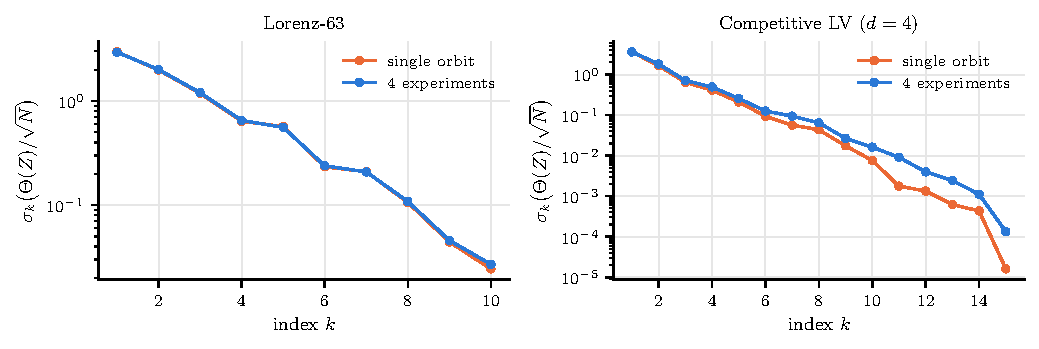
\includegraphics[width=0.9\textwidth]{fig01_library_spectrum}
  \caption{Singular values of the normalised library matrix on noise-free records of equal length, averaged over 5 seeds. Four short perturbed experiments help LV4 by about one order of magnitude in $\sigma_{\min}$, while Lorenz is already well conditioned.}
  \label{fig:spectrum}
\end{figure}

\begin{table}[t]
\centering
\caption{Design ablation at $\dto=\tc/75$: median coefficient error for a single orbit versus four perturbed experiments of the same total length.}
\label{tab:design}
\small
\begin{tabular}{llccccc}
\toprule
system & design & $\varepsilon$ & C1 & C2-FD & C2-SG & C3 \\
\midrule
\multirow{4}{*}{Lorenz} & single orbit & 0\% & 0.018 & 0.0063 & $1.0{\times}10^{-4}$ & $<10^{-6}$ \\
 & 4 experiments & 0\% & 0.013 & 0.0059 & $1.0{\times}10^{-4}$ & $<10^{-6}$ \\
 & single orbit & 1\% & 0.033 & 0.0090 & 0.0075 & 0.0031 \\
 & 4 experiments & 1\% & 0.039 & 0.0067 & 0.0050 & 0.0004 \\
\midrule
\multirow{4}{*}{LV4} & single orbit & 0\% & 0.31 & 0.15 & $1.0{\times}10^{-4}$ & $<10^{-6}$ \\
 & 4 experiments & 0\% & 0.18 & 0.0052 & $4.0{\times}10^{-4}$ & $<10^{-6}$ \\
 & single orbit & 1\% & 3.02 & 2.33 & 3.17 & 2.24 \\
 & 4 experiments & 1\% & 1.63 & 1.56 & 1.06 & 1.53 \\
\bottomrule
\end{tabular}
\end{table}

\section{Classical estimators on the full grid}\label{sec:exp-classical}

\Cref{fig:classical} summarises the classical fits (678 on the main grid, the irregular-sampling condition and the control). On Lorenz-63 the ranking is stable. Weak SINDy is best wherever anything works. Its error at $\varepsilon=1\%$ grows from $4\times10^{-4}$ at $\dto=\tc/75$ to $0.006$ at $\tc/15$ and $0.23$ at $2\tc/15$, and the method fails at $4\tc/15$ ($2.4$). The derivative-based estimators degrade one sampling step earlier. Savitzky--Golay SINDy has error $0.005$ at $\tc/75$, $0.16$ at $\tc/15$ and $1.7$ at $2\tc/15$, close to the $2.9\%$ and $11.7\%$ derivative biases predicted by \eqref{eq:fd}. At the coarsest interval, the estimators that do not diverge collapse onto fixed points or limit cycles: the Benettin exponent of their free runs drops to zero, and $W_1$ rises above one standard deviation. Dense least squares is never competitive.

Two further observations bear on the neural results. First, the weak form is sensitive to the \emph{distribution} of sampling times. With random sampling at the same mean density as $\tc/15$, the largest gaps exceed five times the mean interval, and weak SINDy fails even on noise-free data, whereas finite differences on the non-uniform grid lose accuracy more gracefully (\texttt{classical\_grid.csv}, irregular rows). Second, the failure at coarse sampling is not specific to chaos. On the periodic predator--prey control, every classical estimator has a coefficient error above $0.7$ for $\dto\ge2\tc/15$, including on noise-free data. The limit comes from resolving the signal, not from predictability.

\begin{figure}[t]
  \centering
  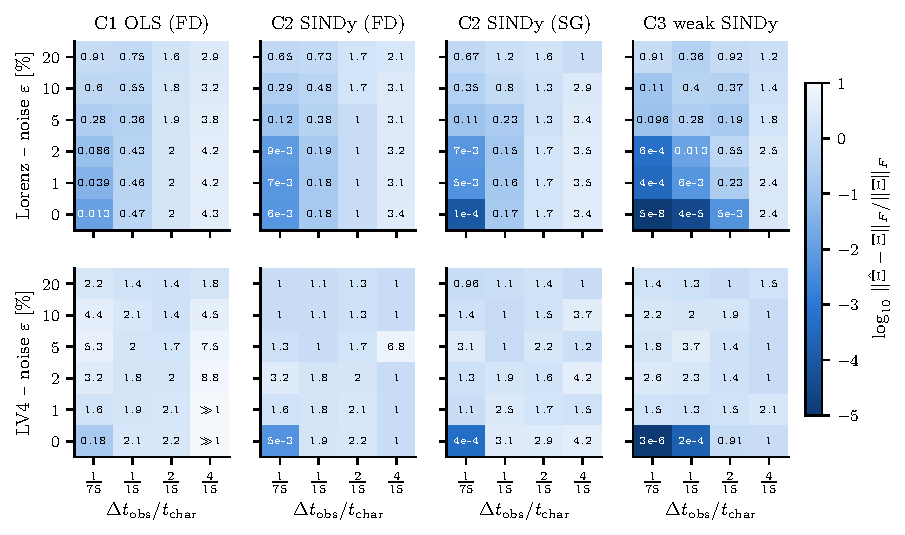
\includegraphics[width=\textwidth]{fig02_classical_heatmaps}
  \caption{Classical estimators: median relative coefficient error over the full sampling $\times$ noise grid (three seeds per cell). Darker is better.}
  \label{fig:classical}
\end{figure}

\section{Benchmark: neural versus classical identification}\label{sec:exp-bench}

\Cref{fig:bench-coef,fig:vpt} and \cref{tab:lorenz,tab:lv4} compare all seven estimators on the cross-shaped sub-grid.

\paragraph{Equation recovery at coarse sampling.} The clearest result concerns the sparse-library model N2 on Lorenz-63 at $\varepsilon=1\%$. Its median coefficient error is $0.009$ at $\dto=\tc/15$, against $0.006$ for weak SINDy. At $2\tc/15$ it is $0.031$, eight times lower than weak SINDy ($0.23$). At $4\tc/15$, where every classical estimator fails ($\ge2.4$), it is $0.052$. On noise-free data at $\tc/15$, N2 recovers the exact support for all seeds with error $<10^{-4}$. For LV4 the same holds without noise (error $10^{-3}$, exact support). Free runs of the N2 models reproduce the invariant statistics as well as the exact equations do: $W_1=0.08$ at $4\tc/15$, compared with $0.08$ for the exact vector field run for the same duration, and an estimated $\lmax=0.93$.

\paragraph{Noise.} At $\dto=\tc/15$ the advantage of N2 shrinks as noise grows. At $2\%$, weak SINDy is slightly better ($0.013$ versus $0.021$). At $5\%$ and $10\%$, N2 is better ($0.09$ versus $0.28$, and $0.21$ versus $0.40$). At $20\%$ no estimator is below a coefficient error of $0.36$. Multiple shooting with latent states performs the denoising, and the integral of the model replaces the integral of the noisy data. Neither helps once the noise standard deviation is comparable to the change of the state over a window.

\paragraph{Black-box model.} The distilled equations of N1 are never competitive. Their errors are between $0.21$ and $1.15$ on Lorenz and above $1.5$ on LV4, with dense supports. As a forecaster, N1 is better than the derivative-based estimators at coarse sampling (VPT $1.1$ versus $\le0.17$ at $4\tc/15$) but worse than the sparse models at fine sampling (VPT $1.2$--$1.8$ against $2.9$--$9.1$ for weak SINDy and N2). Its out-of-distribution VPT is $0.015$ Lyapunov times in every configuration: started off the attractor, the network leaves the observed region of state space immediately and its predictions are meaningless from the first step. Sparse library models with the right support extrapolate correctly by construction. N2 keeps an OOD VPT of $3.3$--$7.1$ on Lorenz at $1\%$ noise across all sampling intervals.

\paragraph{LV4: forecasting despite non-identifiability.} On LV4 at $\varepsilon=1\%$ no estimator recovers the coefficients. Even so, N2 has the longest VPT at every sampling interval: $3.4$ Lyapunov times at $\tc/15$, against $1.4$ for the best classical estimator, and $1.7$ at $4\tc/15$, against $0.16$. Its OOD VPT is $0.65$ against at most $0.06$. Its coefficients are wrong in directions that the attractor does not excite (\cref{sec:exp-data}). Trajectory matching selects among the many equivalent models one that is dynamically consistent with the data, whereas derivative regression amplifies noise along exactly those directions.

\paragraph{Warm starts.} N2-WS, which adds the weak-SINDy estimate to the initialisations, selected that initialisation in 22 of 54 fits, yet its results match N2 to within seed-to-seed variation everywhere. Once the flow-map stage and the continuation are in place, the final model depends little on which of the reasonable starting points is used. This is consistent with the basin study in \cref{sec:exp-landscape}.

\begin{figure}[t]
  \centering
  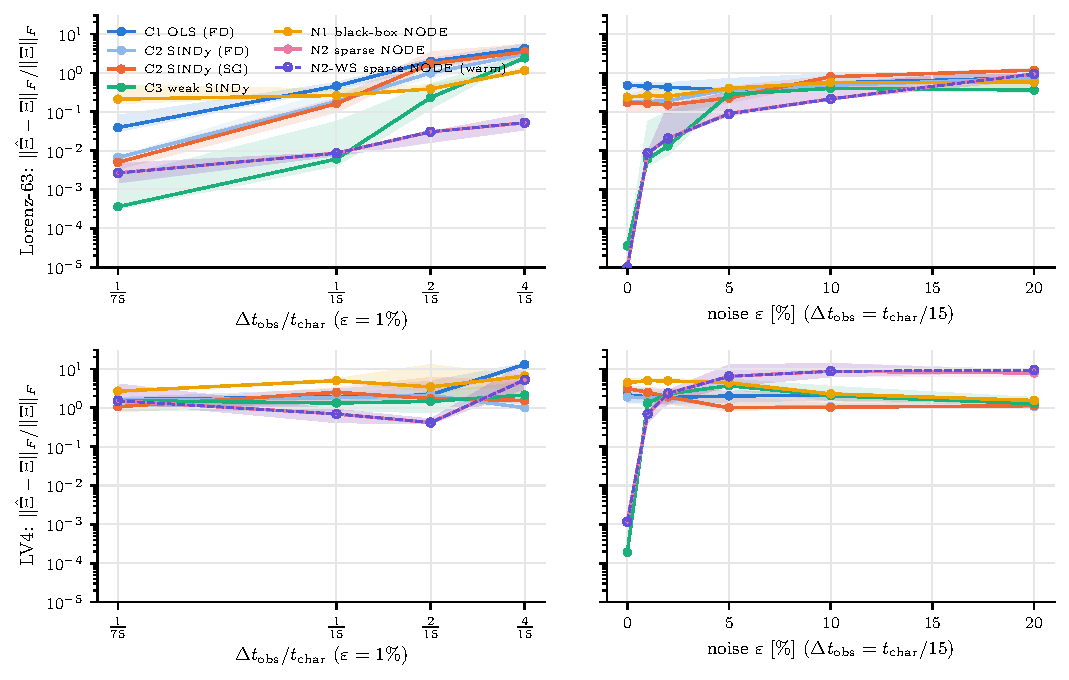
\includegraphics[width=\textwidth]{fig06_benchmark_coef}
  \caption{Coefficient error on the cross-shaped sub-grid: sampling sweep at $\varepsilon=1\%$ (left) and noise sweep at $\dto=\tc/15$ (right). Lines show medians and bands the inter-quartile range over seeds. The N1 curve is for its distilled equations.}
  \label{fig:bench-coef}
\end{figure}

\begin{figure}[t]
  \centering
  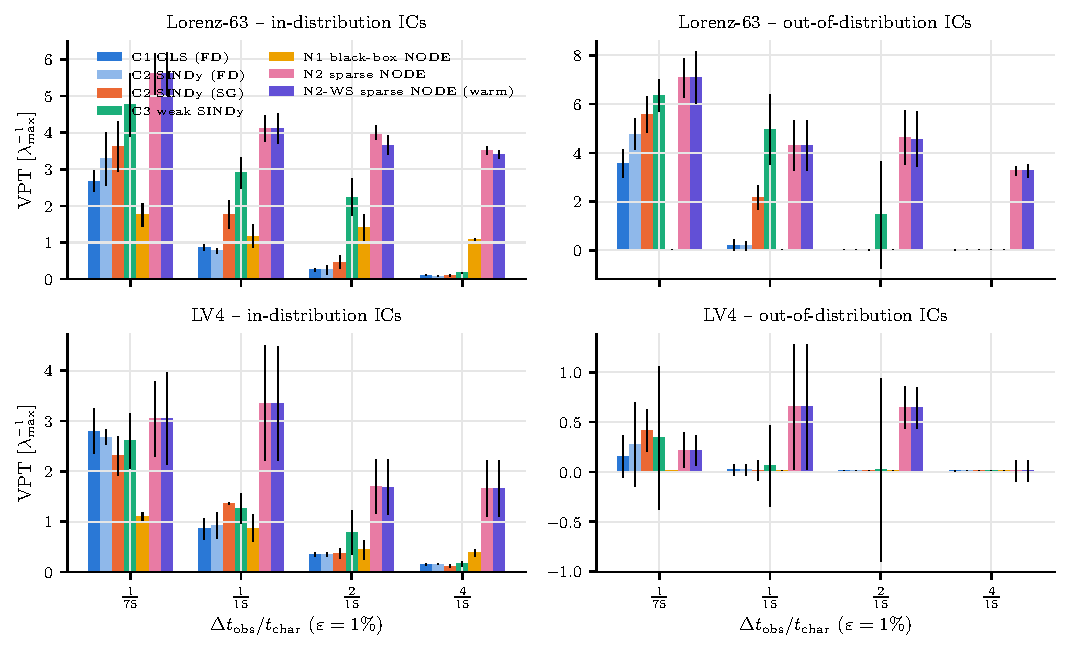
\includegraphics[width=\textwidth]{fig06_vpt}
  \caption{Valid prediction time at $\varepsilon=1\%$ from 16 in-distribution (left) and 16 out-of-distribution (right) initial conditions. Bars show medians over seeds, whiskers the standard deviation. For reference, the exact vector field reaches $11.3$ (Lorenz) and $8.1$ (LV4) in-distribution with the same integrator.}
  \label{fig:vpt}
\end{figure}

\begin{table}[t]
\centering
\caption{Lorenz-63: medians over three seeds in three regimes: \emph{moderate} ($\dto=\tc/15$, $\varepsilon=1\%$), \emph{sparse} ($\dto=4\tc/15$, $\varepsilon=1\%$) and \emph{noisy} ($\dto=\tc/15$, $\varepsilon=10\%$). VPT is in Lyapunov times, $W_1$ in standard deviations; ``--'' marks a divergent free run. $^\dagger$Equation metrics of N1 refer to its distilled equations, forecast metrics to the network.}
\label{tab:lorenz}
\resizebox{\textwidth}{!}{%
\begin{tabular}{l*{15}{c}}
\toprule
 & \multicolumn{5}{c}{moderate} & \multicolumn{5}{c}{sparse} & \multicolumn{5}{c}{noisy} \\
\midrule
 & coef. err. & $F_1$ & VPT$_{\rm ID}$ & VPT$_{\rm OOD}$ & $W_1$ & coef. err. & $F_1$ & VPT$_{\rm ID}$ & VPT$_{\rm OOD}$ & $W_1$ & coef. err. & $F_1$ & VPT$_{\rm ID}$ & VPT$_{\rm OOD}$ & $W_1$ \\
\midrule
C1 OLS (FD) & 0.46 & 0.38 & 0.86 & 0.22 & 0.08 & 4.25 & 0.38 & 0.11 & 0.01 & -- & 0.55 & 0.38 & 0.59 & 0.13 & 0.05 \\
C2 SINDy (FD) & 0.18 & 0.67 & 0.77 & 0.18 & 0.16 & 3.09 & 0.38 & 0.09 & 0.01 & 1.53 & 0.48 & 0.80 & 0.67 & 0.16 & 0.08 \\
C2 SINDy (SG) & 0.16 & 0.64 & 1.77 & 2.18 & 0.11 & 3.47 & 0.39 & 0.09 & 0.01 & 1.53 & 0.80 & 0.48 & 0.68 & 0.14 & 0.11 \\
C3 weak SINDy & 6.1e-3 & 1.00 & 2.90 & 4.96 & 0.14 & 2.43 & 0.46 & 0.17 & 0.01 & 1.11 & 0.40 & 0.48 & 1.66 & 0.06 & 0.14 \\
N1 black-box NODE$^\dagger$ & 0.26 & 0.82 & 1.17 & 0.02 & 0.22 & 1.15 & 0.45 & 1.08 & 0.02 & 0.17 & 0.57 & 0.52 & 1.38 & 0.02 & 0.30 \\
N2 sparse NODE & 8.6e-3 & 1.00 & 4.11 & 4.30 & 0.11 & 0.05 & 0.64 & 3.51 & 3.26 & 0.08 & 0.21 & 0.56 & 1.88 & 0.55 & 0.12 \\
N2-WS (warm start) & 8.6e-3 & 1.00 & 4.11 & 4.30 & 0.17 & 0.05 & 0.64 & 3.40 & 3.26 & 0.08 & 0.21 & 0.56 & 2.03 & 0.99 & 0.05 \\
\bottomrule
\end{tabular}}
\end{table}

\begin{table}[t]
\centering
\caption{Competitive LV ($d=4$), same regimes and conventions as \cref{tab:lorenz}.}
\label{tab:lv4}
\resizebox{\textwidth}{!}{%
\begin{tabular}{l*{15}{c}}
\toprule
 & \multicolumn{5}{c}{moderate} & \multicolumn{5}{c}{sparse} & \multicolumn{5}{c}{noisy} \\
\midrule
 & coef. err. & $F_1$ & VPT$_{\rm ID}$ & VPT$_{\rm OOD}$ & $W_1$ & coef. err. & $F_1$ & VPT$_{\rm ID}$ & VPT$_{\rm OOD}$ & $W_1$ & coef. err. & $F_1$ & VPT$_{\rm ID}$ & VPT$_{\rm OOD}$ & $W_1$ \\
\midrule
C1 OLS (FD) & 1.91 & 0.44 & 0.86 & 0.02 & 0.07 & 13.00 & 0.44 & 0.16 & 0.01 & 0.28 & 2.11 & 0.44 & 0.62 & 0.01 & 0.18 \\
C2 SINDy (FD) & 1.80 & 0.43 & 0.92 & 0.02 & 0.16 & 1.00 & 0.00 & 0.16 & 0.01 & 0.80 & 1.07 & 0.32 & 0.42 & 0.01 & 0.48 \\
C2 SINDy (SG) & 2.51 & 0.43 & 1.36 & 0.01 & 0.24 & 1.54 & 0.00 & 0.12 & 0.01 & 35.94 & 1.03 & 0.40 & 0.58 & 0.01 & 0.80 \\
C3 weak SINDy & 1.32 & 0.48 & 1.26 & 0.06 & 0.08 & 2.13 & 0.21 & 0.16 & 0.01 & 0.80 & 2.04 & 0.42 & 0.29 & 0.01 & 1.18 \\
N1 black-box NODE$^\dagger$ & 4.98 & 0.45 & 0.87 & 0.01 & 0.22 & 6.56 & 0.45 & 0.38 & 0.01 & 0.50 & 2.27 & 0.44 & 0.76 & 0.01 & 0.25 \\
N2 sparse NODE & 0.69 & 0.45 & 3.36 & 0.65 & 0.03 & 5.24 & 0.44 & 1.67 & 0.01 & 0.12 & 8.70 & 0.44 & 0.96 & 0.01 & 0.11 \\
N2-WS (warm start) & 0.69 & 0.45 & 3.36 & 0.65 & 0.03 & 5.24 & 0.44 & 1.67 & 0.01 & 0.12 & 8.70 & 0.44 & 0.96 & 0.01 & 0.11 \\
\bottomrule
\end{tabular}}
\end{table}


\begin{figure}[p]
  \centering
  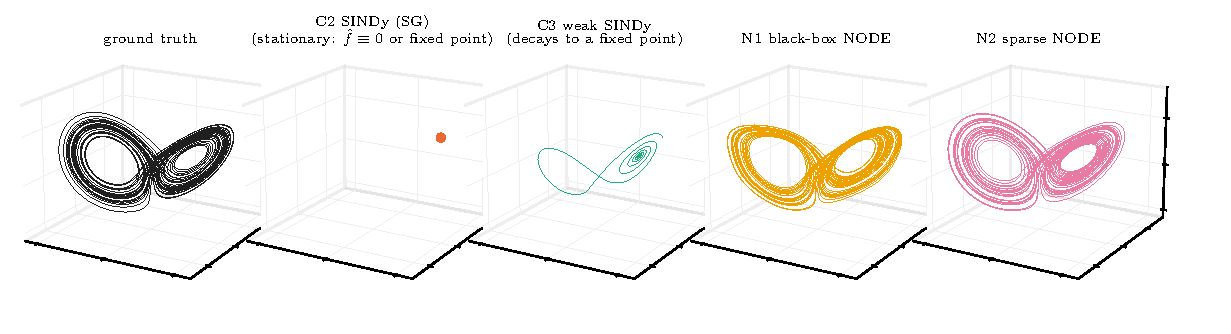
\includegraphics[width=\textwidth]{fig06_gallery_lorenz_dt0.267_n0.01}\\[2pt]
  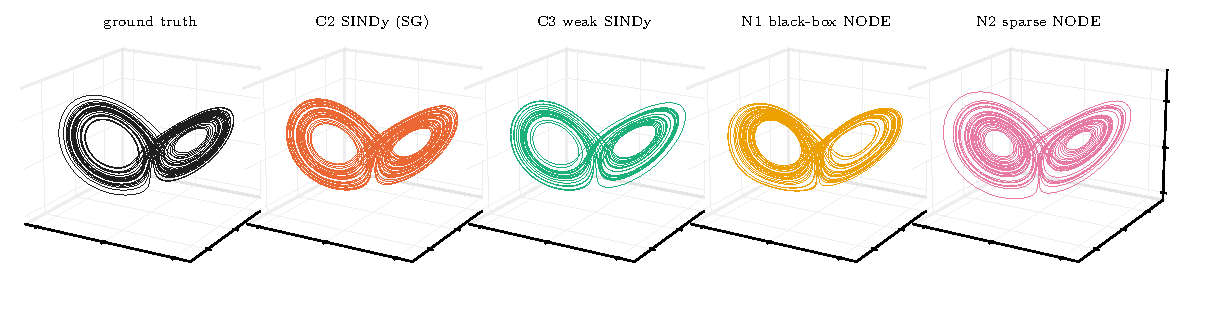
\includegraphics[width=\textwidth]{fig06_gallery_lorenz_dt0.067_n0.05}\\[2pt]
  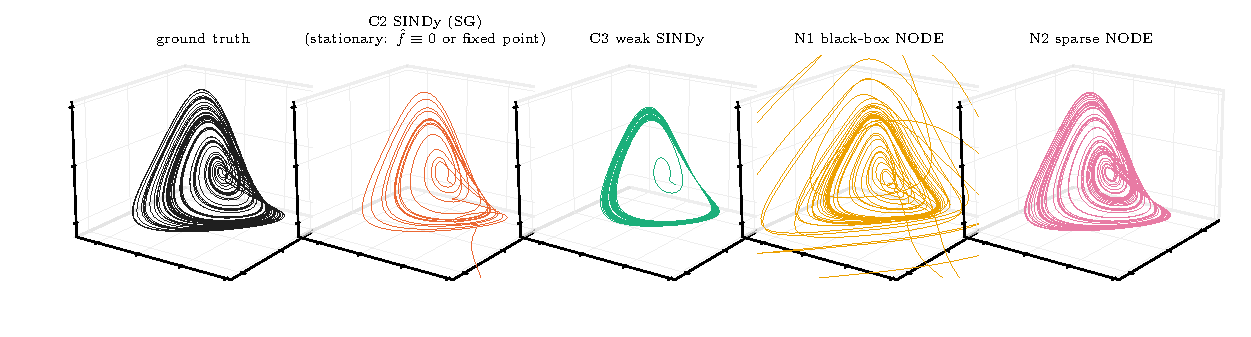
\includegraphics[width=\textwidth]{fig06_gallery_lv4_dt0.067_n0.01}
  \caption{Free runs over $60\tc$ of the identified models (seed 0). Top: Lorenz, $\dto=0.2$, $\varepsilon=1\%$. Middle: Lorenz, $\dto=0.05$, $\varepsilon=5\%$. Bottom: LV4, $\dto=\tc/15$, $\varepsilon=1\%$.}
  \label{fig:gallery}
\end{figure}

\section{Loss landscapes and nonconvex optimisation}\label{sec:exp-landscape}

\paragraph{Exact slices.} \Cref{fig:landscape} shows the trajectory-matching loss of Lorenz-63 as a function of $(\sigma,\rho)$, with $\beta$ at its true value and noise-free data. At $T=0.5$ ($0.45$ Lyapunov times) the single-shooting loss is a smooth valley around the truth. At $T=2$ the valley has narrowed into a curved ridge-bounded channel, and away from it the surface is flat at the level of the attractor's variance. At $T=8$ it is a ``golf course'': almost every parameter value gives the same, maximal loss, and the minimum occupies a thin filament of the grid. The one-dimensional slice in \cref{fig:landscape-slice} makes this precise. For $T=1$ the loss is a smooth funnel. For $T=4$ and $T=8$ it is flat, at the level of the attractor's variance, everywhere except in a dip around $\rho=28$ whose width is a small fraction of a unit. Away from the dip the curve carries irregular small-scale fluctuations: the gradient there is uninformative about the direction of the minimum. The multiple-shooting loss over the same record, with windows of $\tau=0.2$ restarted at the observations, decreases monotonically towards the truth over the whole interval and spans ten decades.

\begin{figure}[t]
  \centering
  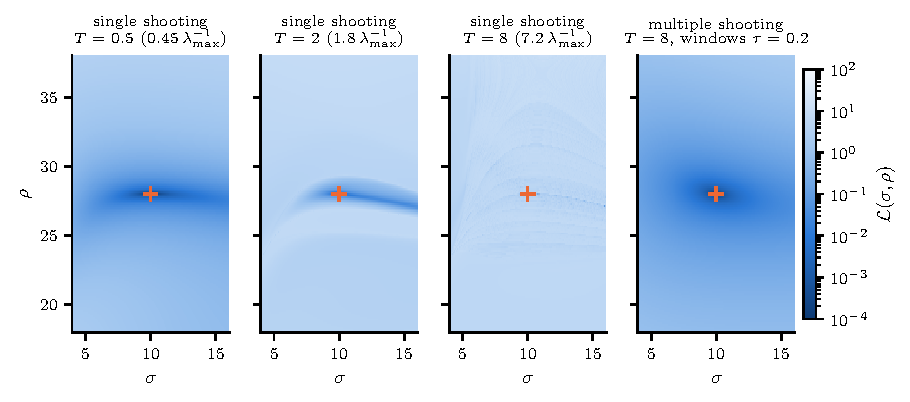
\includegraphics[width=\textwidth]{fig04_landscape_sigma_rho}
  \caption{Trajectory-matching loss $\mathcal L(\sigma,\rho)$ for Lorenz-63 on a $161\times161$ grid, noise-free data, $\beta=8/3$. The cross marks the truth. Single shooting over longer horizons (left three panels) against multiple shooting with $\tau=0.2$ over the longest horizon (right).}
  \label{fig:landscape}
\end{figure}

\begin{figure}[t]
  \centering
  \begin{subfigure}[t]{0.49\textwidth}
    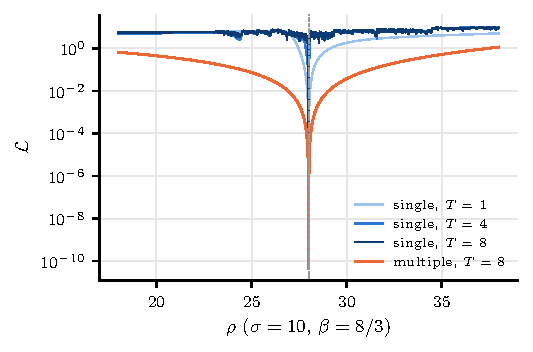
\includegraphics[width=\textwidth]{fig04_landscape_slice}
    \caption{Slice through the truth along $\rho$ (4\,001 points).}
    \label{fig:landscape-slice}
  \end{subfigure}\hfill
  \begin{subfigure}[t]{0.49\textwidth}
    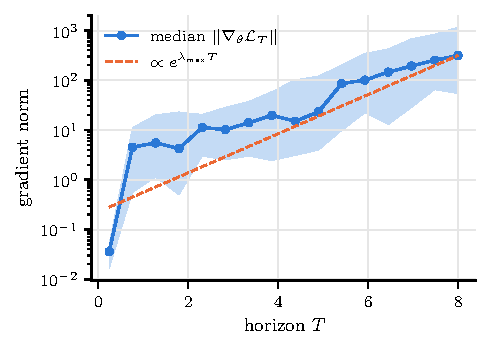
\includegraphics[width=\textwidth]{fig04_gradient_growth}
    \caption{Gradient norm against horizon at 64 points within $\pm5\%$ of the truth (median and 10--90\% band).}
    \label{fig:grad}
  \end{subfigure}
  \caption{Roughness and gradient growth of single shooting.}
\end{figure}

\paragraph{Gradient growth.} \Cref{fig:grad} confirms the mechanism of \cref{prop:basin}. Between $T=2$ and $T=8$ the median gradient norm grows exponentially at a fitted rate of $0.68$, against $\lmax=0.91$. The rate is lower than $\lmax$ for two reasons: the loss averages residuals over the horizon, so early, less sensitive residuals dilute the growth, and the residuals saturate at the size of the attractor once trajectories decorrelate. Over the horizon of $T=8$ the gradient norm still changes by four orders of magnitude, and the 10--90\% band spans more than an order of magnitude at every $T$. No single learning rate is appropriate across horizons, which is the practical side of the roughness.

\paragraph{Basins of attraction (three parameters).} \Cref{fig:basins-param} and \cref{tab:basins} report 96 random restarts of $(\sigma,\rho,\beta)$ estimation from a 1\%-noise record of length 4, using Adam on $\log\theta$.
\begin{itemize}
  \item \emph{Single shooting.} With $T=1$, $42\%$ of the starts reach the truth to within $1\%$. With $T=4$ none do, and only one start in 96 reaches $5\%$.
  \item \emph{Multiple shooting, short windows.} With windows of $K=4$ intervals ($0.2$ time units) and nodes at the observations, all 96 starts converge to the same point, $0.09\%$ from the truth.
  \item \emph{Multiple shooting, long windows.} With $K=20$ ($1$ time unit), all starts again converge to a single point, with or without a $K$-curriculum, but that point is $2.0\%$ from the truth. The noisy observations used as shooting nodes are amplified over the longer windows, and the minimiser itself is biased.
\end{itemize}
Long windows therefore cost accuracy when the nodes are fixed at noisy data. This is the errors-in-variables bias that the latent states $S$ in \eqref{eq:ms} remove.

\begin{table}[t]
\centering
\caption{Random restarts for $(\sigma,\rho,\beta)$: fraction of 96 starts within $1\%$ and $5\%$ of the truth, and median final error.}
\label{tab:basins}
\small
\begin{tabular}{lccc}
\toprule
objective & within 1\% & within 5\% & median error \\
\midrule
single shooting, $T=1$ & 0.42 & 0.42 & 0.34 \\
single shooting, $T=4$ & 0.00 & 0.01 & 0.16 \\
multiple shooting, $K=4$ ($\tau=0.2$) & 1.00 & 1.00 & $8.9\times10^{-4}$ \\
multiple shooting, $K=20$ ($\tau=1$) & 0.00 & 1.00 & 0.020 \\
multiple shooting, $K:1\to20$ & 0.00 & 1.00 & 0.020 \\
\bottomrule
\end{tabular}
\end{table}

\begin{figure}[t]
  \centering
  \begin{subfigure}[t]{0.44\textwidth}
    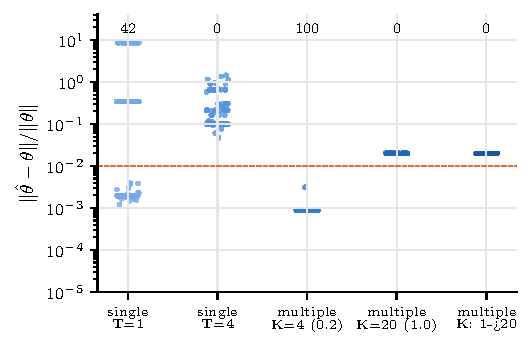
\includegraphics[width=\textwidth]{fig04_basins_parametric}
    \caption{Final relative error of 96 restarts for $(\sigma,\rho,\beta)$. Numbers at the top give the percentage of starts within $1\%$ of the truth (dashed line).}
    \label{fig:basins-param}
  \end{subfigure}\hfill
  \begin{subfigure}[t]{0.54\textwidth}
    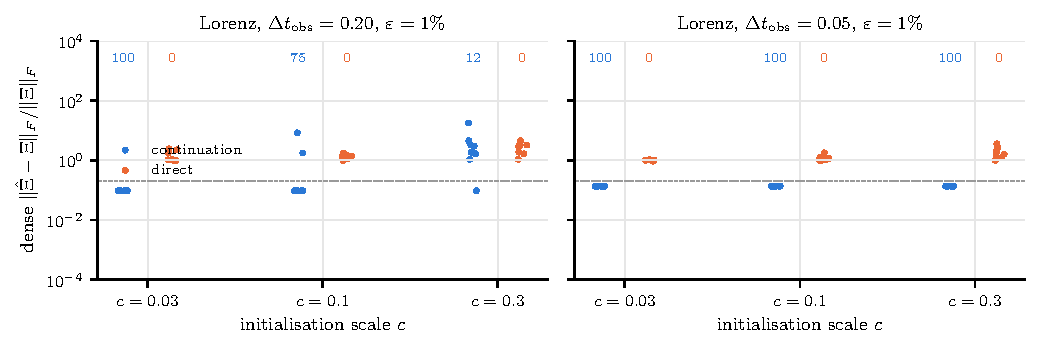
\includegraphics[width=\textwidth]{fig04_basins_library}
    \caption{Random restarts of the 30-coefficient library problem (8 per scale): continuation versus direct training at $K_{\max}$. Numbers at the top give the percentage of runs below the dashed line (dense error $0.2$).}
    \label{fig:basins-lib}
  \end{subfigure}
  \caption{Basins of attraction.}
\end{figure}

\paragraph{Basins of attraction (full library).} \Cref{fig:basins-lib} repeats the experiment for the 30-coefficient library problem with random initialisations $\tilde\Xib_0=c\,\mathcal N(0,\overline{\tilde\Xib_{\rm OLS}^2})$, which use no information about the truth. Training directly at the final window length fails for every start, at every scale and both sampling intervals: none of the 48 runs gets below a dense coefficient error of $0.2$, and most produce non-finite rollouts at the first iteration. With the continuation of \cref{alg:n2}, every start converges at $\dto=0.05$, for all three scales, to the same dense solution, with error $0.14$ before thresholding; after thresholding, the models of the main sweep reach $0.009$ in this configuration. At $\dto=0.2$ the continuation succeeds for $100\%$, $75\%$ and $12\%$ of the starts at $c=0.03$, $0.1$ and $0.3$. The flow-map stage must begin from a field whose one-step map over $\dto=0.2$ stays bounded, and large random quadratic fields do not. This explains why the zero field is the most reliable initialisation in \cref{alg:n2} (selected in 31 of 54 N2 fits), and why multistart over a few such candidates suffices.


\paragraph{The black-box loss surface.} \Cref{fig:nn-landscape} shows filter-normalised slices of the N1 loss around the trained weights. With $K=1$ the trained weights sit at the bottom of a smooth, nearly quadratic bowl ($\log_{10}\mathcal L$ from $-2.9$ at the centre to $-0.5$ at the edges). With $K=15$, the training window, the bowl is narrower and anisotropic and is surrounded by a plateau about three decades higher. With $K=60$ ($4\tc$, close to single shooting) the minimum disappears. The trained weights lie on a broad plateau at the level of the attractor's variance ($\log_{10}\mathcal L\approx 0$), bounded by a cliff where perturbed networks produce unstable trajectories. The long-window objective cannot distinguish the trained model from networks perturbed by half a filter norm. Its gradient carries no information about the short-term dynamics that the model has learned, which is the network analogue of \cref{fig:landscape}.

\begin{figure}[t]
  \centering
  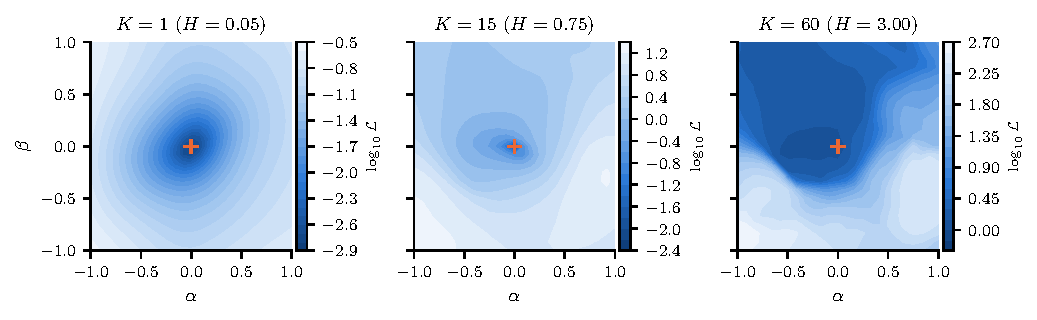
\includegraphics[width=\textwidth]{fig04_nn_landscape}
  \caption{Loss of the trained black-box model (Lorenz, $\dto=0.05$, $\varepsilon=1\%$) on two filter-normalised random directions, evaluated with windows of $K=1$, $15$ and $60$ observation intervals.}
  \label{fig:nn-landscape}
\end{figure}


\section{Uncertainty, stability and out-of-distribution generalisation}\label{sec:exp-uq}

\Cref{tab:uq} scores the four predictive distributions of \cref{sec:uq-theory} at $\dto=\tc/15$ and two noise levels. \Cref{fig:uq-bands} shows typical forecasts, and \cref{fig:uq-cal} the coverage and CRPS against lead time.

\begin{table}[t]
\centering
\caption{Predictive uncertainty at $\dto=\tc/15$, averaged over 16 initial conditions and the first 5 Lyapunov times. Coverage is that of central 90\% intervals (ideal: 0.90). CRPS is in units of $\sigma_i$ (lower is better). The spread--skill column is Spearman's $\rho$ between ensemble spread and the error of the ensemble mean. The shift ratio is the mean spread over the first Lyapunov time for OOD initial conditions divided by that for ID ones.}
\label{tab:uq}
\small
\begin{tabular}{llcccccccc}
\toprule
 & & \multicolumn{2}{c}{coverage} & \multicolumn{2}{c}{CRPS} & \multicolumn{2}{c}{spread--skill} & shift ratio \\
\cmidrule(lr){3-4}\cmidrule(lr){5-6}\cmidrule(lr){7-8}
system, $\varepsilon$ & method & ID & OOD & ID & OOD & ID & OOD & spread / error \\
\midrule
Lorenz, 1\% & E-SINDy (C3) & 0.87 & 0.93 & 0.16 & 0.22 & 0.89 & 0.81 & 15.4 / 20.9 \\
 & N2 bagging & 0.18 & 0.11 & 0.10 & 0.07 & 0.79 & 0.80 & 3.9 / 6.4 \\
 & N1 deep ens. & 0.41 & 0.47 & 0.51 & 1.35 & 0.61 & 0.13 & 11.9 / 23.5 \\
 & N1 MC dropout & 0.67 & 0.64 & 0.64 & 0.96 & 0.21 & -0.09 & 1.1 / 5.3 \\
\midrule
Lorenz, 10\% & E-SINDy (C3) & 0.75 & 0.76 & 0.42 & 0.78 & 0.58 & 0.34 & 11.2 / 10.7 \\
 & N2 bagging & 0.54 & 0.49 & 0.33 & 0.59 & 0.77 & 0.33 & 11.9 / 14.3 \\
 & N1 deep ens. & 0.40 & 0.47 & 0.50 & 0.99 & 0.62 & -0.12 & 9.8 / 17.8 \\
 & N1 MC dropout & 0.68 & 0.65 & 0.62 & 0.89 & 0.23 & -0.14 & 1.0 / 4.9 \\
\midrule
LV4, 1\% & E-SINDy (C3) & 0.95 & 0.95 & 0.57 & 3.31 & 0.68 & 0.53 & 110.1 / 25.6 \\
 & N2 bagging & 0.58 & 0.35 & 0.33 & 3.11 & 0.76 & 0.35 & 125.5 / 142.8 \\
 & N1 deep ens. & 0.38 & 0.47 & 0.65 & 2.65 & 0.25 & 0.10 & 7.4 / 6.8 \\
 & N1 MC dropout & 0.73 & 0.41 & 0.56 & 1.76 & 0.13 & 0.15 & 1.8 / 4.3 \\
\midrule
LV4, 10\% & E-SINDy (C3) & 0.85 & 0.83 & 6.90 & 8.49 & 0.56 & 0.24 & 1.2 / 1.2 \\
 & N2 bagging & 0.50 & 0.17 & 0.65 & 9.96 & 0.47 & 0.28 & 209.4 / 285.8 \\
 & N1 deep ens. & 0.36 & 0.50 & 0.66 & 2.46 & 0.26 & 0.04 & 7.2 / 6.5 \\
 & N1 MC dropout & 0.67 & 0.51 & 0.55 & 1.81 & 0.12 & 0.14 & 2.0 / 4.2 \\
\bottomrule
\end{tabular}
\end{table}

\paragraph{The bootstrap of the weak regression is the best calibrated.} On Lorenz at $1\%$ noise, E-SINDy intervals cover the truth $87\%$ (ID) and $93\%$ (OOD) of the time, against a nominal $90\%$. Their spread is strongly rank-correlated with the actual error ($\rho=0.89$ ID, $0.81$ OOD). The OOD spread is 15 times the ID spread, and the OOD error 21 times the ID error, so the ensemble flags the distribution shift almost in proportion. The calibration survives $10\%$ noise on Lorenz (coverage $0.75$). It breaks down for LV4 at $10\%$, where a few bootstrap members are unstable and inflate both the spread and the CRPS.

\paragraph{Window bagging gives the most accurate but an over-confident distribution.} N2 has the lowest CRPS in five of the eight comparisons; the exceptions are LV4 out of distribution and LV4 at $10\%$ noise in distribution, where the black-box ensembles are best. Its spread is informative (spread--skill $0.79$--$0.80$ on Lorenz at $1\%$) but far too small: the members are nearly identical, and coverage is only $0.18$ ID and $0.11$ OOD. Resampling windows perturbs a problem that the continuation solves almost deterministically, so the bootstrap explores a single basin. Its intervals need recalibration, for instance by inflating the spread on held-out data, before they can be read as probabilities.

\paragraph{Deep ensembles detect the shift; MC dropout does not.} For the black-box model, the deep ensemble's spread grows about tenfold out of distribution ($11.9\times$ on Lorenz at 1\%), which correctly signals that the forecasts should not be trusted. Its spread--skill correlation, however, drops from $0.61$ to $0.13$, and coverage stays below $0.5$. MC dropout with trajectory-wise masks produces a spread that is almost independent of the initial condition (ratio $1.0$--$2.0$), while its error grows four- to fivefold out of distribution. It also degrades the median forecast, which drifts away from the truth within one Lyapunov time even in distribution (\cref{fig:uq-bands}). In our setting dropout gives neither an accurate forecaster nor a useful detector of distribution shift.

\begin{figure}[t]
  \centering
  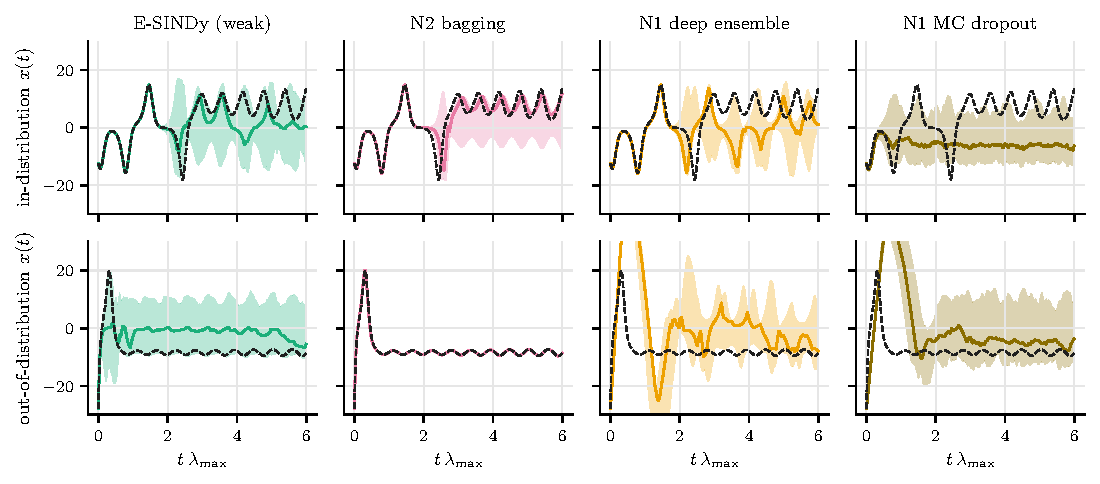
\includegraphics[width=\textwidth]{fig05_uq_bands}
  \caption{Forecasts of $x(t)$ for Lorenz ($\dto=0.05$, $\varepsilon=1\%$) from an in-distribution (top) and an out-of-distribution (bottom) initial condition. Lines show the median of the ensemble, bands the 5--95\% range, and the dashed line the truth.}
  \label{fig:uq-bands}
\end{figure}

\begin{figure}[t]
  \centering
  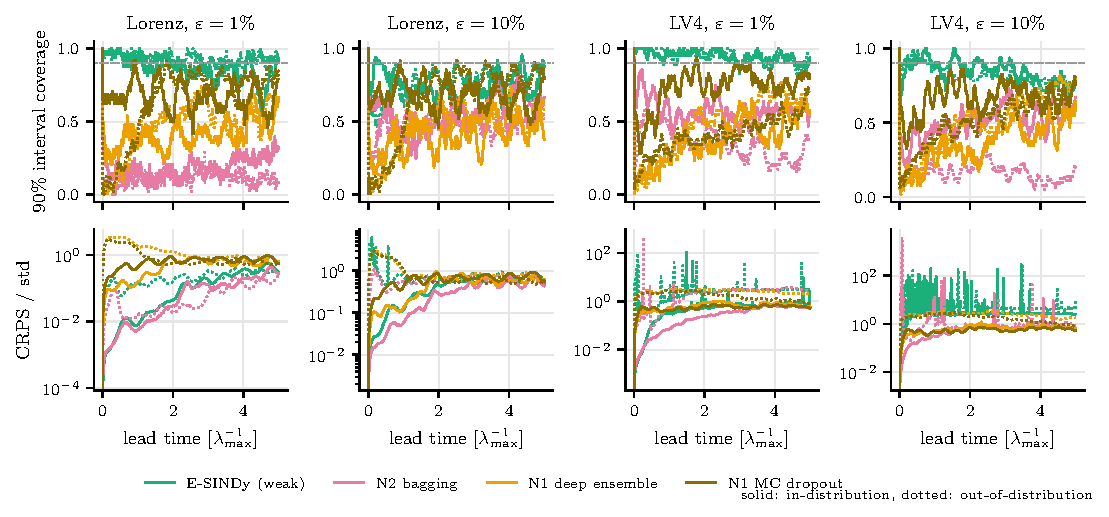
\includegraphics[width=\textwidth]{fig05_uq_calibration}
  \caption{Coverage of central 90\% intervals (top) and CRPS (bottom) against lead time, for in-distribution (solid) and out-of-distribution (dotted) initial conditions.}
  \label{fig:uq-cal}
\end{figure}

\paragraph{Uncertainty in the support.} \Cref{fig:inclusion} shows E-SINDy inclusion probabilities on Lorenz across noise levels. The true terms are kept in essentially every bootstrap sample up to $10\%$ noise. At $20\%$ the selected threshold rises and some true terms of the $\dot x$ and $\dot z$ equations are dropped in about half of the samples. The spurious terms behave differently in the three equations. The $\dot z$ equation stays clean up to $2\%$. In the $\dot x$ and $\dot y$ equations, spurious monomials appear in 10--25\% of the samples even without noise, in 30--60\% at $1$--$2\%$, and in almost all samples at $5$--$10\%$, although the point estimate has the exact support at low noise. The bootstrap is therefore more pessimistic than the point estimate. It locates the doubt in the equations where the library is nearly degenerate on the data: $x$ and $y$ are strongly correlated on the attractor, since $\dot x=\sigma(y-x)$ is small compared with $x$, and the constant, $z$ and $z^2$ columns are nearly collinear because $z$ stays far from zero.

\begin{figure}[t]
  \centering
  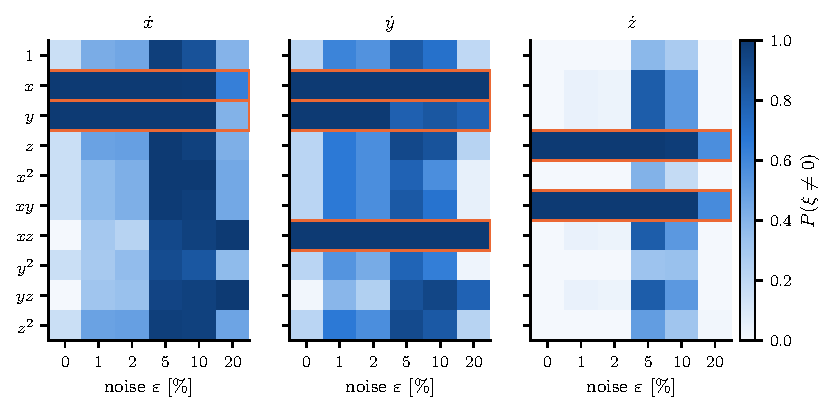
\includegraphics[width=\textwidth]{fig05_inclusion}
  \caption{E-SINDy inclusion probabilities $P(\xi_{kj}\neq0)$ for Lorenz at $\dto=0.05$ across noise levels (100 bootstrap samples). True terms are outlined.}
  \label{fig:inclusion}
\end{figure}


\section{Discussion}\label{sec:discussion}

\paragraph{When do neural models help?} The answer depends on what ``neural'' means. Integration through a differentiable solver brings a real gain over derivative-based and weak-form regression in one regime, coarse sampling at low noise. That gain is obtained by the sparse-library model, whose function class is the same as SINDy's. The black-box network adds nothing for equation discovery. It forecasts in-distribution only moderately, and it fails out of distribution without exception. The benefit therefore comes from the objective, matching trajectories instead of derivatives, and not from neural function approximation. Without the optimisation devices of \cref{sec:tm} this benefit is unreachable. Single shooting fails beyond about one Lyapunov time, and the flow-map stage needs a starting field whose one-step map is finite.

\paragraph{When does nothing help?} On the four-species LV model, coefficient recovery fails for every estimator as soon as the data are noisy. The singular values of the library show why: the attractor does not excite all directions of coefficient space, and four perturbed experiments improve $\sigma_{\min}$ by only an order of magnitude. The useful question is then not which estimator to use but which data to collect. Experiments that start further from the attractor, or interventions that drive the system through other regimes, would be needed. Short-term forecasts remain possible, and trajectory matching provides the best of them.

\paragraph{Limitations.}
\begin{itemize}
  \item The library contains the true model. Library misspecification, partial observation and coloured noise are not studied.
  \item The neural estimators were run on a sub-grid with three seeds. The GPU notebook extends this to the full grid with five seeds.
  \item N2 is more expensive than weak SINDy, by one to two orders of magnitude in wall-clock time.
  \item Its bagging ensemble is over-confident and would need recalibration before its intervals are read as probabilities.
  \item The noise levels are relative to the attractor's standard deviation. For LV4, whose library is badly conditioned, even $1\%$ is beyond what any estimator can handle.
\end{itemize}


\chapter{Conclusion}\label{ch:conclusion}

This report compared classical and neural approaches to discovering and forecasting chaotic dynamics from short, sparse and noisy records, with the sampling interval as the primary experimental axis. Four conclusions stand out.

\begin{enumerate}
  \item \textbf{Integration-based sparse identification extends equation discovery to coarse sampling.} With multiple shooting, joint state estimation, continuation from a one-step flow-map regression and multistart, a sparse-library neural ODE recovers the Lorenz-63 equations from records with about four samples per oscillation and $1\%$ noise (median coefficient error $0.05$). At that sampling every derivative-based and weak-form estimator fails. At two-thirds of that interval it is eight times more accurate than weak SINDy.
  \item \textbf{The optimisation devices are necessary, and their necessity is measurable.} Exact loss slices show single shooting turning into a flat surface with a needle-like minimum. Gradient norms grow exponentially with the horizon, at a rate of $0.68$ against $\lmax=0.91$. Short-window multiple shooting brings all random restarts to the same accurate solution, while single shooting over four time units brings none.
  \item \textbf{Black-box neural ODEs are poor tools for discovery and do not extrapolate.} Their distilled equations are dense and inaccurate. Their forecasts fail immediately from initial conditions away from the attractor, although deep ensembles at least signal this with a tenfold increase in spread. Monte Carlo dropout does not.
  \item \textbf{Identifiability is a property of the data.} For the four-species LV model, the library is so badly conditioned on the attractor that no estimator recovers the coefficients from noisy data. Trajectory matching still yields the most accurate forecasts there, by selecting a dynamically consistent model among nearly equivalent ones.
\end{enumerate}

For uncertainty, the bootstrap of the weak regression was the best calibrated (coverage $0.87$--$0.93$ against a nominal $0.90$). Window bagging of the sparse NODE gave the lowest CRPS but intervals that are far too narrow. A natural next step is to combine the two: integration-based estimates for accuracy, with recalibrated or Bayesian dispersion for honest intervals. Further steps are to replace the fixed monomial library by a learnable or misspecified one, and to design experiments that improve the conditioning of the library before the data are collected.

\paragraph{Code and data.} All results are produced by six executed Jupyter notebooks (Python, NumPy, SciPy, PyTorch). Every number in this report is exported to CSV in \texttt{results/metrics}.


\appendix
\chapter{Hyper-parameters}\label{app:hyper}

\begin{table}[h]
\centering
\caption{Settings shared by all experiments.}
\small
\resizebox{\textwidth}{!}{%
\begin{tabular}{ll}
\toprule
item & value \\
\midrule
ground truth & DOP853, $\mathrm{rtol}=10^{-10}$, $\mathrm{atol}=10^{-12}$, grid $\tc/750$ \\
record & 4 experiments $\times\ \tfrac{20}{3}\tc$; initial-state perturbation $0.5\sigma_i$; 80/20 split \\
rollouts of learned models & classical RK4, $h=\tc/75$; divergence if $\norm{x}>10^4$ \\
model selection & rollouts of $\tc$ from 24 held-out observations; rel.\ tol.\ 5\%, abs.\ tol.\ $10^{-4}$ \\
STLSQ & 24 thresholds in $[10^{-4},10^{-0.3}]\max|\tilde\Xib_{\rm OLS}|$; ridge $10^{-10}$; $\le25$ sweeps \\
Savitzky--Golay & cubic; $w\in\{5,7,9,13,17,25\}$ \\
weak form & $\phi=(1-s^2)^4$; $H\in\{0.1,0.2,0.35,0.5,0.75\}\tc$, $H\ge2\dto$ \\
N1 network & $\tanh$, $2\times64$; output layer scaled by $0.1$ at initialisation \\
N1 training & Adam; lr $3\cdot10^{-3}$ (states $10^{-2}$), decay $0.6$/stage, cosine in last stage \\
 & batch 128 windows; clip 1; $w=0.5$; $H\in\{0.1,0.25,0.5,1\}\tc$, $\{200,250,300,450\}$ it. \\
N1 dropout (UQ) & $p=0.1$ on hidden units, mask fixed per trajectory, 30 samples \\
N2 flow-map stage & Levenberg--Marquardt, 50 it., $\mu_0=10^{-3}$, Marquardt scaling \\
N2 multiple shooting & L-BFGS (history 20, strong Wolfe), 60 it.\ per stage; $K=1,2,3,5,8,\dots,K_{\max}$ \\
 & $K_{\max}\dto\approx\tc$; $\le2048$ windows; $w=0.5$ \\
N2 thresholding & 12 values in $[10^{-3},10^{-0.4}]\max|\tilde\Xib|$; $\le4$ sweeps; L-BFGS refits (15 it., 256 windows) \\
ensembles & 5 members (N1 deep ensemble, N2 window bagging); E-SINDy 100 bootstraps \\
test sets & 16 ID + 16 OOD initial conditions; horizon 15 Lyapunov times; free runs $200\tc$ \\
\bottomrule
\end{tabular}}
\end{table}

\chapter{Additional results}\label{app:extra}

\section{Recovered equations at coarse sampling}

Lorenz-63, $\varepsilon=1\%$, seed 0 (true model: $\dot x=-10x+10y$, $\dot y=28x-y-xz$, $\dot z=-\tfrac83z+xy$).

\medskip
\noindent\textbf{$\dto=0.1$.} Weak SINDy and N2 both find the exact support at this seed. The median over seeds, $0.23$ for weak SINDy against $0.03$ for N2, reflects the other seeds.
\begin{align*}
\text{C3:}\quad & \dot x=-9.944x+9.945y,\quad \dot y=28.163x-1.074y-1.003xz,\\ & \dot z=-2.659z+0.998xy\\
\text{N2:}\quad & \dot x=-10.016x+10.060y,\quad \dot y=27.956x-1.005y-0.999xz,\\ & \dot z=-2.663z+0.997xy
\end{align*}
\noindent\textbf{$\dto=0.2$.}
\begin{align*}
\text{C3:}\quad & \dot x=-14.797x+13.943y+0.199xz-0.195yz\\
& \dot y=-24.998-7.239x+12.332y+2.864z\\
& \qquad\ +0.340xy-0.267y^2-0.236yz-0.067z^2\\
& \dot z=-57.602+8.993z+3.363x^2-2.242xy+0.595y^2-0.433z^2\\
\text{N2:}\quad & \dot x=-9.587x+9.727y-0.021xz+0.017yz\\
& \dot y=28.025x-1.018y-1.000xz,\qquad \dot z=-2.655z+1.000xy
\end{align*}
At $\dto=0.2$ the N2 model contains two spurious terms with coefficients of order $10^{-2}$, and its free runs are indistinguishable from the true attractor (\cref{fig:gallery}). The distilled N1 equations at this sampling are dense, with 26 of 30 possible terms active.

\section{Observation records in phase space}

\begin{figure}[h]
  \centering
  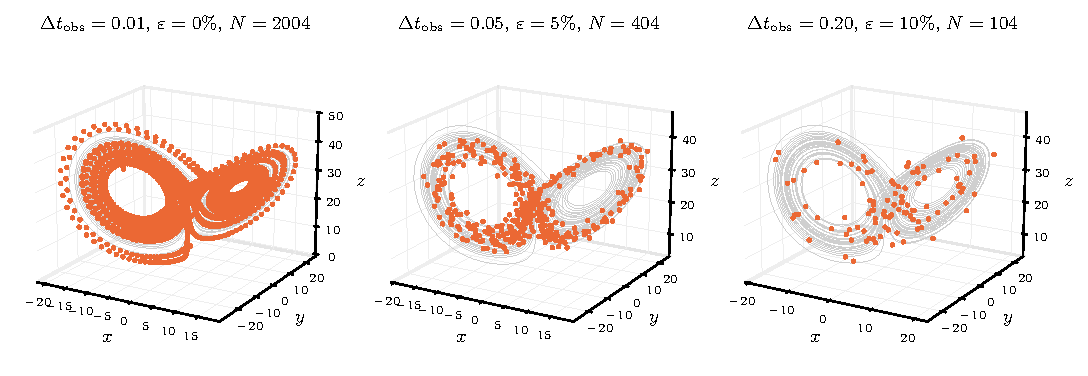
\includegraphics[width=\textwidth]{fig01_samples_phase_space}
  \caption{Lorenz-63 observations (all four experiments, seed 0) at three corruption levels, over the reference attractor.}
\end{figure}

\section{Training dynamics}

\begin{figure}[h]
  \centering
  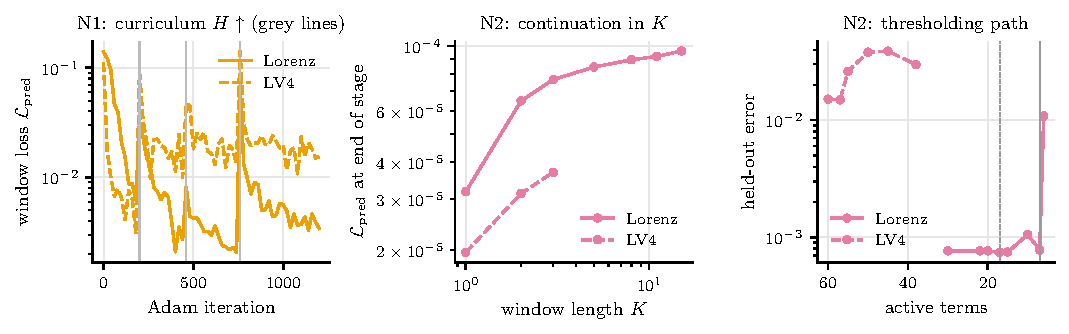
\includegraphics[width=\textwidth]{fig03_training}
  \caption{Left: N1 window loss during the curriculum ($\dto=\tc/15$, $\varepsilon=1\%$). Centre: N2 window loss at the end of each continuation stage. Right: held-out error along the N2 thresholding path; vertical lines mark the true number of active terms.}
\end{figure}


\footnotesize
\printbibliography[heading=bibintoc,title={References}]
\normalsize

\end{document}
